\documentclass[twoside]{book}

% Packages required by doxygen
\usepackage{fixltx2e}
\usepackage{calc}
\usepackage{doxygen}
\usepackage[export]{adjustbox} % also loads graphicx
\usepackage{graphicx}
\usepackage[utf8]{inputenc}
\usepackage{makeidx}
\usepackage{multicol}
\usepackage{multirow}
\PassOptionsToPackage{warn}{textcomp}
\usepackage{textcomp}
\usepackage[nointegrals]{wasysym}
\usepackage[table]{xcolor}

% Font selection
\usepackage[T1]{fontenc}
\usepackage[scaled=.90]{helvet}
\usepackage{courier}
\usepackage{amssymb}
\usepackage{sectsty}
\renewcommand{\familydefault}{\sfdefault}
\allsectionsfont{%
  \fontseries{bc}\selectfont%
  \color{darkgray}%
}
\renewcommand{\DoxyLabelFont}{%
  \fontseries{bc}\selectfont%
  \color{darkgray}%
}
\newcommand{\+}{\discretionary{\mbox{\scriptsize$\hookleftarrow$}}{}{}}

% Page & text layout
\usepackage{geometry}
\geometry{%
  a4paper,%
  top=2.5cm,%
  bottom=2.5cm,%
  left=2.5cm,%
  right=2.5cm%
}
\tolerance=750
\hfuzz=15pt
\hbadness=750
\setlength{\emergencystretch}{15pt}
\setlength{\parindent}{0cm}
\setlength{\parskip}{3ex plus 2ex minus 2ex}
\makeatletter
\renewcommand{\paragraph}{%
  \@startsection{paragraph}{4}{0ex}{-1.0ex}{1.0ex}{%
    \normalfont\normalsize\bfseries\SS@parafont%
  }%
}
\renewcommand{\subparagraph}{%
  \@startsection{subparagraph}{5}{0ex}{-1.0ex}{1.0ex}{%
    \normalfont\normalsize\bfseries\SS@subparafont%
  }%
}
\makeatother

% Headers & footers
\usepackage{fancyhdr}
\pagestyle{fancyplain}
\fancyhead[LE]{\fancyplain{}{\bfseries\thepage}}
\fancyhead[CE]{\fancyplain{}{}}
\fancyhead[RE]{\fancyplain{}{\bfseries\leftmark}}
\fancyhead[LO]{\fancyplain{}{\bfseries\rightmark}}
\fancyhead[CO]{\fancyplain{}{}}
\fancyhead[RO]{\fancyplain{}{\bfseries\thepage}}
\fancyfoot[LE]{\fancyplain{}{}}
\fancyfoot[CE]{\fancyplain{}{}}
\fancyfoot[RE]{\fancyplain{}{\bfseries\scriptsize Generated by Doxygen }}
\fancyfoot[LO]{\fancyplain{}{\bfseries\scriptsize Generated by Doxygen }}
\fancyfoot[CO]{\fancyplain{}{}}
\fancyfoot[RO]{\fancyplain{}{}}
\renewcommand{\footrulewidth}{0.4pt}
\renewcommand{\chaptermark}[1]{%
  \markboth{#1}{}%
}
\renewcommand{\sectionmark}[1]{%
  \markright{\thesection\ #1}%
}

% Indices & bibliography
\usepackage{natbib}
\usepackage[titles]{tocloft}
\setcounter{tocdepth}{3}
\setcounter{secnumdepth}{5}
\makeindex

% Hyperlinks (required, but should be loaded last)
\usepackage{ifpdf}
\ifpdf
  \usepackage[pdftex,pagebackref=true]{hyperref}
\else
  \usepackage[ps2pdf,pagebackref=true]{hyperref}
\fi
\hypersetup{%
  colorlinks=true,%
  linkcolor=blue,%
  citecolor=blue,%
  unicode%
}

% Custom commands
\newcommand{\clearemptydoublepage}{%
  \newpage{\pagestyle{empty}\cleardoublepage}%
}

\usepackage{caption}
\captionsetup{labelsep=space,justification=centering,font={bf},singlelinecheck=off,skip=4pt,position=top}

%===== C O N T E N T S =====

\begin{document}

% Titlepage & ToC
\hypersetup{pageanchor=false,
             bookmarksnumbered=true,
             pdfencoding=unicode
            }
\pagenumbering{roman}
\begin{titlepage}
\vspace*{7cm}
\begin{center}%
{\Large Projet\+Techno\+L3\+T\+P1 \\[1ex]\large 0.\+0.\+1 }\\
\vspace*{1cm}
{\large Generated by Doxygen 1.8.11}\\
\end{center}
\end{titlepage}
\clearemptydoublepage
\tableofcontents
\clearemptydoublepage
\pagenumbering{arabic}
\hypersetup{pageanchor=true}

%--- Begin generated contents ---
\chapter{Class Index}
\section{Class List}
Here are the classes, structs, unions and interfaces with brief descriptions\+:\begin{DoxyCompactList}
\item\contentsline{section}{\hyperlink{structei__app__event__t}{ei\+\_\+app\+\_\+event\+\_\+t} \\*The event parameter for application defined event types }{\pageref{structei__app__event__t}}{}
\item\contentsline{section}{\hyperlink{structei__color__t}{ei\+\_\+color\+\_\+t} \\*A color with transparency }{\pageref{structei__color__t}}{}
\item\contentsline{section}{\hyperlink{structei__display__event__t}{ei\+\_\+display\+\_\+event\+\_\+t} \\*The event parameter for display-\/related event types }{\pageref{structei__display__event__t}}{}
\item\contentsline{section}{\hyperlink{structei__event__t}{ei\+\_\+event\+\_\+t} \\*Describes an event }{\pageref{structei__event__t}}{}
\item\contentsline{section}{\hyperlink{structei__key__event__t}{ei\+\_\+key\+\_\+event\+\_\+t} \\*The event parameter for keyboard-\/related event types }{\pageref{structei__key__event__t}}{}
\item\contentsline{section}{\hyperlink{structei__linked__point__t}{ei\+\_\+linked\+\_\+point\+\_\+t} \\*A point plus a pointer to create a linked list }{\pageref{structei__linked__point__t}}{}
\item\contentsline{section}{\hyperlink{structei__linked__rect__t}{ei\+\_\+linked\+\_\+rect\+\_\+t} \\*A rectangle plus a pointer to create a linked list }{\pageref{structei__linked__rect__t}}{}
\item\contentsline{section}{\hyperlink{structei__linked__tag__t}{ei\+\_\+linked\+\_\+tag\+\_\+t} \\*A tag and a pointer to create a linked list }{\pageref{structei__linked__tag__t}}{}
\item\contentsline{section}{\hyperlink{structei__mouse__event__t}{ei\+\_\+mouse\+\_\+event\+\_\+t} \\*The event parameter for mouse-\/related event types }{\pageref{structei__mouse__event__t}}{}
\item\contentsline{section}{\hyperlink{structei__point__t}{ei\+\_\+point\+\_\+t} \\*A 2-\/D point with integer coordinates }{\pageref{structei__point__t}}{}
\item\contentsline{section}{\hyperlink{structei__rect__t}{ei\+\_\+rect\+\_\+t} \\*A rectangle defined by its top-\/left corner, and its size }{\pageref{structei__rect__t}}{}
\item\contentsline{section}{\hyperlink{structei__size__t}{ei\+\_\+size\+\_\+t} \\*A 2-\/D size with integer dimensions }{\pageref{structei__size__t}}{}
\item\contentsline{section}{\hyperlink{structei__touch__event__t}{ei\+\_\+touch\+\_\+event\+\_\+t} \\*The event parameter for mouse-\/related event types }{\pageref{structei__touch__event__t}}{}
\end{DoxyCompactList}

\chapter{File Index}
\section{File List}
Here is a list of all documented files with brief descriptions\+:\begin{DoxyCompactList}
\item\contentsline{section}{include/\hyperlink{ei__event_8h}{ei\+\_\+event.\+h} \\*Allows the binding and unbinding of callbacks to events }{\pageref{ei__event_8h}}{}
\item\contentsline{section}{include/\hyperlink{ei__main_8h}{ei\+\_\+main.\+h} \\*Declares the \char`\"{}ei\+\_\+main\char`\"{} function\+: the main function of programs built with the libei }{\pageref{ei__main_8h}}{}
\item\contentsline{section}{include/\hyperlink{ei__types_8h}{ei\+\_\+types.\+h} \\*Type, constant, and global definitions for the ei library }{\pageref{ei__types_8h}}{}
\item\contentsline{section}{include/\hyperlink{hw__interface_8h}{hw\+\_\+interface.\+h} \\*Low level interface with the graphic hadware. This interface is based on the S\+DL library }{\pageref{hw__interface_8h}}{}
\end{DoxyCompactList}

\chapter{Class Documentation}
\hypertarget{structei__app__event__t}{}\section{ei\+\_\+app\+\_\+event\+\_\+t Struct Reference}
\label{structei__app__event__t}\index{ei\+\_\+app\+\_\+event\+\_\+t@{ei\+\_\+app\+\_\+event\+\_\+t}}


The event parameter for application defined event types.  




{\ttfamily \#include $<$ei\+\_\+event.\+h$>$}

\subsection*{Public Attributes}
\begin{DoxyCompactItemize}
\item 
void $\ast$ {\bfseries user\+\_\+param}\hypertarget{structei__app__event__t_a236a89c3726aa9c770da42ba37ce3d3f}{}\label{structei__app__event__t_a236a89c3726aa9c770da42ba37ce3d3f}

\end{DoxyCompactItemize}


\subsection{Detailed Description}
The event parameter for application defined event types. 

The documentation for this struct was generated from the following file\+:\begin{DoxyCompactItemize}
\item 
include/\hyperlink{ei__event_8h}{ei\+\_\+event.\+h}\end{DoxyCompactItemize}

\hypertarget{structei__color__t}{}\section{ei\+\_\+color\+\_\+t Struct Reference}
\label{structei__color__t}\index{ei\+\_\+color\+\_\+t@{ei\+\_\+color\+\_\+t}}


A color with transparency.  




{\ttfamily \#include $<$ei\+\_\+types.\+h$>$}

\subsection*{Public Attributes}
\begin{DoxyCompactItemize}
\item 
unsigned char \hyperlink{structei__color__t_a9adf283c79176b3426ac63784f0bc17b}{red}\hypertarget{structei__color__t_a9adf283c79176b3426ac63784f0bc17b}{}\label{structei__color__t_a9adf283c79176b3426ac63784f0bc17b}

\begin{DoxyCompactList}\small\item\em The red component of the color. \end{DoxyCompactList}\item 
unsigned char \hyperlink{structei__color__t_ad85ce262fb9c76fe3c52b4eed19505d1}{green}\hypertarget{structei__color__t_ad85ce262fb9c76fe3c52b4eed19505d1}{}\label{structei__color__t_ad85ce262fb9c76fe3c52b4eed19505d1}

\begin{DoxyCompactList}\small\item\em The green component of the color. \end{DoxyCompactList}\item 
unsigned char \hyperlink{structei__color__t_af8d67b7a72cbb586519b55033350fb8c}{blue}\hypertarget{structei__color__t_af8d67b7a72cbb586519b55033350fb8c}{}\label{structei__color__t_af8d67b7a72cbb586519b55033350fb8c}

\begin{DoxyCompactList}\small\item\em The blue component of the color. \end{DoxyCompactList}\item 
unsigned char \hyperlink{structei__color__t_af213a14356db920b1a04f5270263ae61}{alpha}
\end{DoxyCompactItemize}


\subsection{Detailed Description}
A color with transparency. 

Each channel is represented as an 8 bits unsigned interger, hence channel\textquotesingle{}s minimum value is 0, maximum is 255. 

\subsection{Member Data Documentation}
\index{ei\+\_\+color\+\_\+t@{ei\+\_\+color\+\_\+t}!alpha@{alpha}}
\index{alpha@{alpha}!ei\+\_\+color\+\_\+t@{ei\+\_\+color\+\_\+t}}
\subsubsection[{\texorpdfstring{alpha}{alpha}}]{\setlength{\rightskip}{0pt plus 5cm}unsigned char ei\+\_\+color\+\_\+t\+::alpha}\hypertarget{structei__color__t_af213a14356db920b1a04f5270263ae61}{}\label{structei__color__t_af213a14356db920b1a04f5270263ae61}
The transparency of the color. 0 is invisible, 

The documentation for this struct was generated from the following file\+:\begin{DoxyCompactItemize}
\item 
include/\hyperlink{ei__types_8h}{ei\+\_\+types.\+h}\end{DoxyCompactItemize}

\hypertarget{structei__display__event__t}{}\section{ei\+\_\+display\+\_\+event\+\_\+t Struct Reference}
\label{structei__display__event__t}\index{ei\+\_\+display\+\_\+event\+\_\+t@{ei\+\_\+display\+\_\+event\+\_\+t}}


The event parameter for display-\/related event types.  




{\ttfamily \#include $<$ei\+\_\+event.\+h$>$}

\subsection*{Public Attributes}
\begin{DoxyCompactItemize}
\item 
\hyperlink{ei__types_8h_a383b9af13bd6a0a893096ead3c4d8e28}{ei\+\_\+bool\+\_\+t} \hyperlink{structei__display__event__t_a32e23d401fad708e99701cde6d30e9d9}{resized}\hypertarget{structei__display__event__t_a32e23d401fad708e99701cde6d30e9d9}{}\label{structei__display__event__t_a32e23d401fad708e99701cde6d30e9d9}

\begin{DoxyCompactList}\small\item\em The window has been resized. \end{DoxyCompactList}\item 
\hyperlink{ei__types_8h_a383b9af13bd6a0a893096ead3c4d8e28}{ei\+\_\+bool\+\_\+t} \hyperlink{structei__display__event__t_a29dcb5bdf052575615f3566839c630ce}{closed}\hypertarget{structei__display__event__t_a29dcb5bdf052575615f3566839c630ce}{}\label{structei__display__event__t_a29dcb5bdf052575615f3566839c630ce}

\begin{DoxyCompactList}\small\item\em The close button of the window has been pressed. \end{DoxyCompactList}\item 
\hyperlink{ei__types_8h_a383b9af13bd6a0a893096ead3c4d8e28}{ei\+\_\+bool\+\_\+t} \hyperlink{structei__display__event__t_ae688be60429c4516a9ba9a0813902252}{switched\+\_\+out}\hypertarget{structei__display__event__t_ae688be60429c4516a9ba9a0813902252}{}\label{structei__display__event__t_ae688be60429c4516a9ba9a0813902252}

\begin{DoxyCompactList}\small\item\em The window is no longer active. \end{DoxyCompactList}\item 
\hyperlink{ei__types_8h_a383b9af13bd6a0a893096ead3c4d8e28}{ei\+\_\+bool\+\_\+t} \hyperlink{structei__display__event__t_a42bd677878c67d8b4262b0e3db22fbc8}{switched\+\_\+in}\hypertarget{structei__display__event__t_a42bd677878c67d8b4262b0e3db22fbc8}{}\label{structei__display__event__t_a42bd677878c67d8b4262b0e3db22fbc8}

\begin{DoxyCompactList}\small\item\em The window is active once again. \end{DoxyCompactList}\end{DoxyCompactItemize}


\subsection{Detailed Description}
The event parameter for display-\/related event types. 

The documentation for this struct was generated from the following file\+:\begin{DoxyCompactItemize}
\item 
include/\hyperlink{ei__event_8h}{ei\+\_\+event.\+h}\end{DoxyCompactItemize}

\hypertarget{structei__event__t}{}\section{ei\+\_\+event\+\_\+t Struct Reference}
\label{structei__event__t}\index{ei\+\_\+event\+\_\+t@{ei\+\_\+event\+\_\+t}}


Describes an event.  




{\ttfamily \#include $<$ei\+\_\+event.\+h$>$}



Collaboration diagram for ei\+\_\+event\+\_\+t\+:
\nopagebreak
\begin{figure}[H]
\begin{center}
\leavevmode
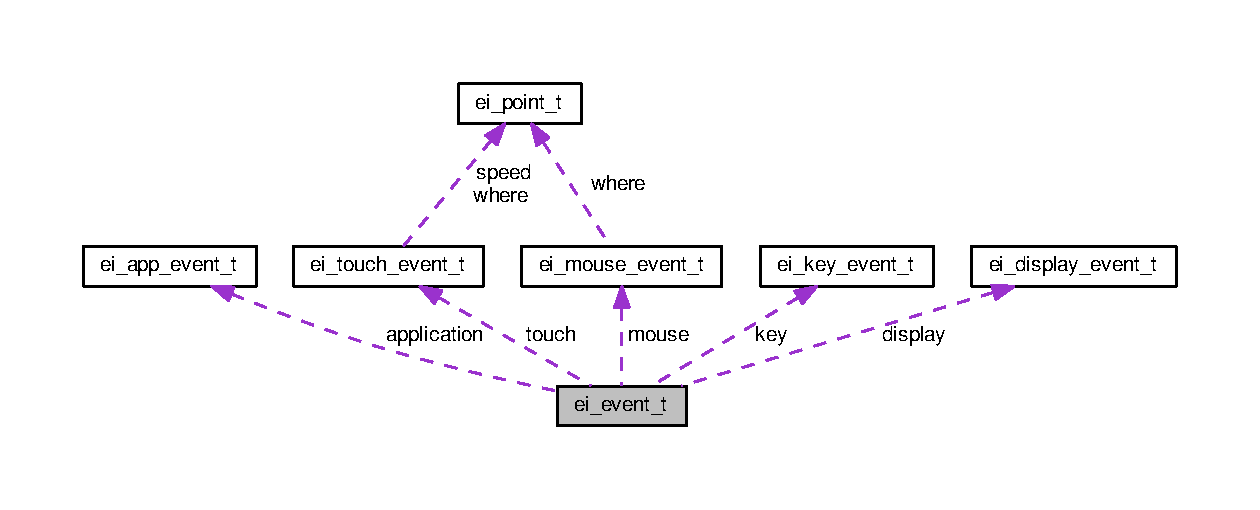
\includegraphics[width=350pt]{structei__event__t__coll__graph}
\end{center}
\end{figure}
\subsection*{Public Attributes}
\begin{DoxyCompactItemize}
\item 
\hyperlink{ei__event_8h_a132dde064150d861ad24e9d839cbe007}{ei\+\_\+eventtype\+\_\+t} \hyperlink{structei__event__t_aee18f11986ed603959de628558812c58}{type}\hypertarget{structei__event__t_aee18f11986ed603959de628558812c58}{}\label{structei__event__t_aee18f11986ed603959de628558812c58}

\begin{DoxyCompactList}\small\item\em The type of the event. \end{DoxyCompactList}\item 
\begin{tabbing}
xx\=xx\=xx\=xx\=xx\=xx\=xx\=xx\=xx\=\kill
union \{\\
\>\hyperlink{structei__display__event__t}{ei\_display\_event\_t} \hyperlink{structei__event__t_aa0c523780572b4ea92fb3f9a016f6c04}{display}\\
\>\>{\em Event parameter for display-\/realted events (see \hyperlink{structei__display__event__t}{ei\_display\_event\_t}). }\\
\>\hyperlink{structei__key__event__t}{ei\_key\_event\_t} \hyperlink{structei__event__t_a0f146bb41b78f27e18ecccc71f50026d}{key}\\
\>\>{\em Event parameters for keyboard-\/related events (see \hyperlink{structei__key__event__t}{ei\_key\_event\_t}). }\\
\>\hyperlink{structei__mouse__event__t}{ei\_mouse\_event\_t} \hyperlink{structei__event__t_a7f0b0d0cf765a822aca7a435510d9d85}{mouse}\\
\>\>{\em Event parameters for mouse-\/related events (see \hyperlink{structei__mouse__event__t}{ei\_mouse\_event\_t}). }\\
\>\hyperlink{structei__touch__event__t}{ei\_touch\_event\_t} \hyperlink{structei__event__t_a8f3c33a53f2738bd153c923b3a6ad20d}{touch}\\
\>\>{\em Event parameters for touch-\/related events (see \hyperlink{structei__touch__event__t}{ei\_touch\_event\_t}). }\\
\>\hyperlink{structei__app__event__t}{ei\_app\_event\_t} \hyperlink{structei__event__t_ab93b7dc04597613a3bd0195e74a9f7bb}{application}\\
\>\>{\em Event parameters for application-\/related events (see \hyperlink{structei__app__event__t}{ei\_app\_event\_t}). }\\
\} {\bfseries param}\hypertarget{structei__event__t_a03a01773dff790d4b772f6b16e4fbb4b}{}\label{structei__event__t_a03a01773dff790d4b772f6b16e4fbb4b}
\\

\end{tabbing}\end{DoxyCompactItemize}


\subsection{Detailed Description}
Describes an event. 

The documentation for this struct was generated from the following file\+:\begin{DoxyCompactItemize}
\item 
include/\hyperlink{ei__event_8h}{ei\+\_\+event.\+h}\end{DoxyCompactItemize}

\hypertarget{structei__key__event__t}{}\section{ei\+\_\+key\+\_\+event\+\_\+t Struct Reference}
\label{structei__key__event__t}\index{ei\+\_\+key\+\_\+event\+\_\+t@{ei\+\_\+key\+\_\+event\+\_\+t}}


The event parameter for keyboard-\/related event types.  




{\ttfamily \#include $<$ei\+\_\+event.\+h$>$}

\subsection*{Public Attributes}
\begin{DoxyCompactItemize}
\item 
int \hyperlink{structei__key__event__t_a55a3611e3a15b95b21be4218f7fa6f3d}{key\+\_\+sym}\hypertarget{structei__key__event__t_a55a3611e3a15b95b21be4218f7fa6f3d}{}\label{structei__key__event__t_a55a3611e3a15b95b21be4218f7fa6f3d}

\begin{DoxyCompactList}\small\item\em The keyboard key symbol (see allegro5/keycodes.\+h). \end{DoxyCompactList}\item 
int \hyperlink{structei__key__event__t_a85ecd793d10f4314b1ac8f2f46c52c88}{unichar}\hypertarget{structei__key__event__t_a85ecd793d10f4314b1ac8f2f46c52c88}{}\label{structei__key__event__t_a85ecd793d10f4314b1ac8f2f46c52c88}

\begin{DoxyCompactList}\small\item\em For \hyperlink{ei__event_8h_a132dde064150d861ad24e9d839cbe007a65746b5440ecd78bceecfaad7ee107ad}{ei\+\_\+ev\+\_\+keychar}, a Unicode code point (character). \end{DoxyCompactList}\item 
\hyperlink{ei__event_8h_abcdd2ef0f39179463f17a06be9bdf949}{ei\+\_\+modifier\+\_\+mask\+\_\+t} \hyperlink{structei__key__event__t_a35e4dc6d788b9fdd4eeedf716662afab}{modifier\+\_\+mask}\hypertarget{structei__key__event__t_a35e4dc6d788b9fdd4eeedf716662afab}{}\label{structei__key__event__t_a35e4dc6d788b9fdd4eeedf716662afab}

\begin{DoxyCompactList}\small\item\em The state of the modifier keys at the time of the event. \end{DoxyCompactList}\end{DoxyCompactItemize}


\subsection{Detailed Description}
The event parameter for keyboard-\/related event types. 

The documentation for this struct was generated from the following file\+:\begin{DoxyCompactItemize}
\item 
include/\hyperlink{ei__event_8h}{ei\+\_\+event.\+h}\end{DoxyCompactItemize}

\hypertarget{structei__linked__point__t}{}\section{ei\+\_\+linked\+\_\+point\+\_\+t Struct Reference}
\label{structei__linked__point__t}\index{ei\+\_\+linked\+\_\+point\+\_\+t@{ei\+\_\+linked\+\_\+point\+\_\+t}}


A point plus a pointer to create a linked list.  




{\ttfamily \#include $<$ei\+\_\+types.\+h$>$}



Collaboration diagram for ei\+\_\+linked\+\_\+point\+\_\+t\+:\nopagebreak
\begin{figure}[H]
\begin{center}
\leavevmode
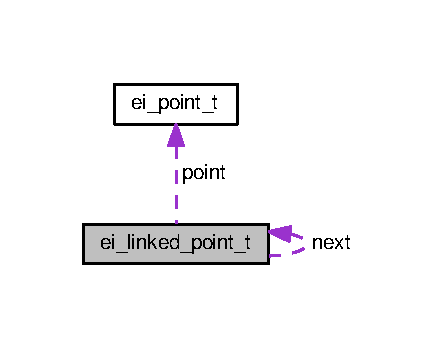
\includegraphics[width=209pt]{structei__linked__point__t__coll__graph}
\end{center}
\end{figure}
\subsection*{Public Attributes}
\begin{DoxyCompactItemize}
\item 
\hyperlink{structei__point__t}{ei\+\_\+point\+\_\+t} \hyperlink{structei__linked__point__t_a5774a3902514ef5c0f599829894c56a6}{point}\hypertarget{structei__linked__point__t_a5774a3902514ef5c0f599829894c56a6}{}\label{structei__linked__point__t_a5774a3902514ef5c0f599829894c56a6}

\begin{DoxyCompactList}\small\item\em The point. \end{DoxyCompactList}\item 
struct \hyperlink{structei__linked__point__t}{ei\+\_\+linked\+\_\+point\+\_\+t} $\ast$ \hyperlink{structei__linked__point__t_aa629ae723d95d2b5538d95306579443c}{next}\hypertarget{structei__linked__point__t_aa629ae723d95d2b5538d95306579443c}{}\label{structei__linked__point__t_aa629ae723d95d2b5538d95306579443c}

\begin{DoxyCompactList}\small\item\em The pointer to the next element in the linked list. \end{DoxyCompactList}\end{DoxyCompactItemize}


\subsection{Detailed Description}
A point plus a pointer to create a linked list. 

The documentation for this struct was generated from the following file\+:\begin{DoxyCompactItemize}
\item 
include/\hyperlink{ei__types_8h}{ei\+\_\+types.\+h}\end{DoxyCompactItemize}

\hypertarget{structei__linked__rect__t}{}\section{ei\+\_\+linked\+\_\+rect\+\_\+t Struct Reference}
\label{structei__linked__rect__t}\index{ei\+\_\+linked\+\_\+rect\+\_\+t@{ei\+\_\+linked\+\_\+rect\+\_\+t}}


A rectangle plus a pointer to create a linked list.  




{\ttfamily \#include $<$ei\+\_\+types.\+h$>$}



Collaboration diagram for ei\+\_\+linked\+\_\+rect\+\_\+t\+:\nopagebreak
\begin{figure}[H]
\begin{center}
\leavevmode
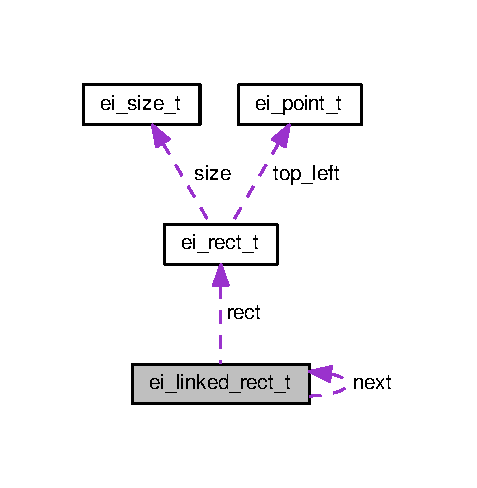
\includegraphics[width=229pt]{structei__linked__rect__t__coll__graph}
\end{center}
\end{figure}
\subsection*{Public Attributes}
\begin{DoxyCompactItemize}
\item 
\hyperlink{structei__rect__t}{ei\+\_\+rect\+\_\+t} \hyperlink{structei__linked__rect__t_ae7fa184a482756ca81a340de0775cc8b}{rect}\hypertarget{structei__linked__rect__t_ae7fa184a482756ca81a340de0775cc8b}{}\label{structei__linked__rect__t_ae7fa184a482756ca81a340de0775cc8b}

\begin{DoxyCompactList}\small\item\em The rectangle. \end{DoxyCompactList}\item 
struct \hyperlink{structei__linked__rect__t}{ei\+\_\+linked\+\_\+rect\+\_\+t} $\ast$ \hyperlink{structei__linked__rect__t_ad31a83bb4babee5aaae18ccedad52755}{next}\hypertarget{structei__linked__rect__t_ad31a83bb4babee5aaae18ccedad52755}{}\label{structei__linked__rect__t_ad31a83bb4babee5aaae18ccedad52755}

\begin{DoxyCompactList}\small\item\em The pointer to the next element in the linked list. \end{DoxyCompactList}\end{DoxyCompactItemize}


\subsection{Detailed Description}
A rectangle plus a pointer to create a linked list. 

The documentation for this struct was generated from the following file\+:\begin{DoxyCompactItemize}
\item 
include/\hyperlink{ei__types_8h}{ei\+\_\+types.\+h}\end{DoxyCompactItemize}

\hypertarget{structei__linked__tag__t}{}\section{ei\+\_\+linked\+\_\+tag\+\_\+t Struct Reference}
\label{structei__linked__tag__t}\index{ei\+\_\+linked\+\_\+tag\+\_\+t@{ei\+\_\+linked\+\_\+tag\+\_\+t}}


A tag and a pointer to create a linked list.  




{\ttfamily \#include $<$ei\+\_\+event.\+h$>$}



Collaboration diagram for ei\+\_\+linked\+\_\+tag\+\_\+t\+:
\nopagebreak
\begin{figure}[H]
\begin{center}
\leavevmode
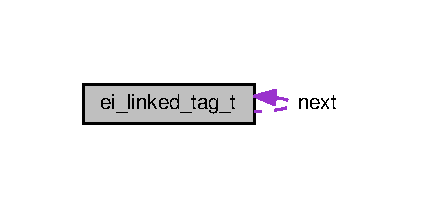
\includegraphics[width=202pt]{structei__linked__tag__t__coll__graph}
\end{center}
\end{figure}
\subsection*{Public Attributes}
\begin{DoxyCompactItemize}
\item 
\hyperlink{ei__event_8h_a24a8242260cfd8ddb6ef915f3de5a10f}{ei\+\_\+tag\+\_\+t} {\bfseries tag}\hypertarget{structei__linked__tag__t_aa1c771b8b7ac760ee10d33d5a29c97d7}{}\label{structei__linked__tag__t_aa1c771b8b7ac760ee10d33d5a29c97d7}

\item 
struct \hyperlink{structei__linked__tag__t}{ei\+\_\+linked\+\_\+tag\+\_\+t} $\ast$ {\bfseries next}\hypertarget{structei__linked__tag__t_a86bfd7536ee8b26a3f2b1a46562591e4}{}\label{structei__linked__tag__t_a86bfd7536ee8b26a3f2b1a46562591e4}

\end{DoxyCompactItemize}


\subsection{Detailed Description}
A tag and a pointer to create a linked list. 

The documentation for this struct was generated from the following file\+:\begin{DoxyCompactItemize}
\item 
include/\hyperlink{ei__event_8h}{ei\+\_\+event.\+h}\end{DoxyCompactItemize}

\hypertarget{structei__mouse__event__t}{}\section{ei\+\_\+mouse\+\_\+event\+\_\+t Struct Reference}
\label{structei__mouse__event__t}\index{ei\+\_\+mouse\+\_\+event\+\_\+t@{ei\+\_\+mouse\+\_\+event\+\_\+t}}


The event parameter for mouse-\/related event types.  




{\ttfamily \#include $<$ei\+\_\+event.\+h$>$}



Collaboration diagram for ei\+\_\+mouse\+\_\+event\+\_\+t\+:
\nopagebreak
\begin{figure}[H]
\begin{center}
\leavevmode
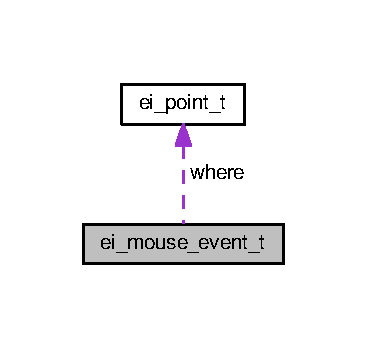
\includegraphics[width=176pt]{structei__mouse__event__t__coll__graph}
\end{center}
\end{figure}
\subsection*{Public Attributes}
\begin{DoxyCompactItemize}
\item 
\hyperlink{structei__point__t}{ei\+\_\+point\+\_\+t} \hyperlink{structei__mouse__event__t_ac50f216f7af2a99469bd39cebc309af5}{where}\hypertarget{structei__mouse__event__t_ac50f216f7af2a99469bd39cebc309af5}{}\label{structei__mouse__event__t_ac50f216f7af2a99469bd39cebc309af5}

\begin{DoxyCompactList}\small\item\em Where the mouse pointer was at the time of the event. \end{DoxyCompactList}\item 
int \hyperlink{structei__mouse__event__t_a3165d2e07c861aa9ccb114a10a6b0afb}{button\+\_\+number}
\end{DoxyCompactItemize}


\subsection{Detailed Description}
The event parameter for mouse-\/related event types. 

\subsection{Member Data Documentation}
\index{ei\+\_\+mouse\+\_\+event\+\_\+t@{ei\+\_\+mouse\+\_\+event\+\_\+t}!button\+\_\+number@{button\+\_\+number}}
\index{button\+\_\+number@{button\+\_\+number}!ei\+\_\+mouse\+\_\+event\+\_\+t@{ei\+\_\+mouse\+\_\+event\+\_\+t}}
\subsubsection[{\texorpdfstring{button\+\_\+number}{button_number}}]{\setlength{\rightskip}{0pt plus 5cm}int ei\+\_\+mouse\+\_\+event\+\_\+t\+::button\+\_\+number}\hypertarget{structei__mouse__event__t_a3165d2e07c861aa9ccb114a10a6b0afb}{}\label{structei__mouse__event__t_a3165d2e07c861aa9ccb114a10a6b0afb}
The number of the button that was pressed or released. 

The documentation for this struct was generated from the following file\+:\begin{DoxyCompactItemize}
\item 
include/\hyperlink{ei__event_8h}{ei\+\_\+event.\+h}\end{DoxyCompactItemize}

\hypertarget{structei__point__t}{}\section{ei\+\_\+point\+\_\+t Struct Reference}
\label{structei__point__t}\index{ei\+\_\+point\+\_\+t@{ei\+\_\+point\+\_\+t}}


A 2-\/D point with integer coordinates.  




{\ttfamily \#include $<$ei\+\_\+types.\+h$>$}

\subsection*{Public Attributes}
\begin{DoxyCompactItemize}
\item 
int \hyperlink{structei__point__t_a6ec4a8846bae4b9694506dae039047b3}{x}\hypertarget{structei__point__t_a6ec4a8846bae4b9694506dae039047b3}{}\label{structei__point__t_a6ec4a8846bae4b9694506dae039047b3}

\begin{DoxyCompactList}\small\item\em The abscissa of the point. The origin is on the left side of the image. \end{DoxyCompactList}\item 
int \hyperlink{structei__point__t_a0c0f1bfa95c372595c52522877f556a0}{y}
\end{DoxyCompactItemize}


\subsection{Detailed Description}
A 2-\/D point with integer coordinates. 

\subsection{Member Data Documentation}
\index{ei\+\_\+point\+\_\+t@{ei\+\_\+point\+\_\+t}!y@{y}}
\index{y@{y}!ei\+\_\+point\+\_\+t@{ei\+\_\+point\+\_\+t}}
\subsubsection[{\texorpdfstring{y}{y}}]{\setlength{\rightskip}{0pt plus 5cm}int ei\+\_\+point\+\_\+t\+::y}\hypertarget{structei__point__t_a0c0f1bfa95c372595c52522877f556a0}{}\label{structei__point__t_a0c0f1bfa95c372595c52522877f556a0}
The ordinate of the point, the origin is at the top of the image, 

The documentation for this struct was generated from the following file\+:\begin{DoxyCompactItemize}
\item 
include/\hyperlink{ei__types_8h}{ei\+\_\+types.\+h}\end{DoxyCompactItemize}

\hypertarget{structei__rect__t}{}\section{ei\+\_\+rect\+\_\+t Struct Reference}
\label{structei__rect__t}\index{ei\+\_\+rect\+\_\+t@{ei\+\_\+rect\+\_\+t}}


A rectangle defined by its top-\/left corner, and its size.  




{\ttfamily \#include $<$ei\+\_\+types.\+h$>$}



Collaboration diagram for ei\+\_\+rect\+\_\+t\+:
\nopagebreak
\begin{figure}[H]
\begin{center}
\leavevmode
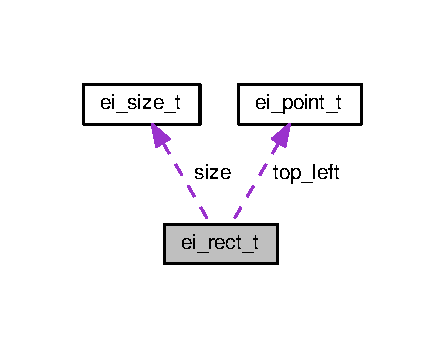
\includegraphics[width=214pt]{structei__rect__t__coll__graph}
\end{center}
\end{figure}
\subsection*{Public Attributes}
\begin{DoxyCompactItemize}
\item 
\hyperlink{structei__point__t}{ei\+\_\+point\+\_\+t} \hyperlink{structei__rect__t_aabe78780aa971b9cb9742ed59a2e9438}{top\+\_\+left}\hypertarget{structei__rect__t_aabe78780aa971b9cb9742ed59a2e9438}{}\label{structei__rect__t_aabe78780aa971b9cb9742ed59a2e9438}

\begin{DoxyCompactList}\small\item\em Coordinates of the top-\/left corner of the rectangle. \end{DoxyCompactList}\item 
\hyperlink{structei__size__t}{ei\+\_\+size\+\_\+t} \hyperlink{structei__rect__t_a200c48a352d448a24d4f85673f6bad14}{size}\hypertarget{structei__rect__t_a200c48a352d448a24d4f85673f6bad14}{}\label{structei__rect__t_a200c48a352d448a24d4f85673f6bad14}

\begin{DoxyCompactList}\small\item\em Size of the rectangle. \end{DoxyCompactList}\end{DoxyCompactItemize}


\subsection{Detailed Description}
A rectangle defined by its top-\/left corner, and its size. 

The documentation for this struct was generated from the following file\+:\begin{DoxyCompactItemize}
\item 
include/\hyperlink{ei__types_8h}{ei\+\_\+types.\+h}\end{DoxyCompactItemize}

\hypertarget{structei__size__t}{}\section{ei\+\_\+size\+\_\+t Struct Reference}
\label{structei__size__t}\index{ei\+\_\+size\+\_\+t@{ei\+\_\+size\+\_\+t}}


A 2-\/D size with integer dimensions.  




{\ttfamily \#include $<$ei\+\_\+types.\+h$>$}

\subsection*{Public Attributes}
\begin{DoxyCompactItemize}
\item 
int {\bfseries width}\hypertarget{structei__size__t_a981037618942814a4318a4c27cdaecc1}{}\label{structei__size__t_a981037618942814a4318a4c27cdaecc1}

\item 
int {\bfseries height}\hypertarget{structei__size__t_a2f152e26c90d01cac2b337ebc118a5f1}{}\label{structei__size__t_a2f152e26c90d01cac2b337ebc118a5f1}

\end{DoxyCompactItemize}


\subsection{Detailed Description}
A 2-\/D size with integer dimensions. 

The documentation for this struct was generated from the following file\+:\begin{DoxyCompactItemize}
\item 
include/\hyperlink{ei__types_8h}{ei\+\_\+types.\+h}\end{DoxyCompactItemize}

\hypertarget{structei__touch__event__t}{}\section{ei\+\_\+touch\+\_\+event\+\_\+t Struct Reference}
\label{structei__touch__event__t}\index{ei\+\_\+touch\+\_\+event\+\_\+t@{ei\+\_\+touch\+\_\+event\+\_\+t}}


The event parameter for mouse-\/related event types.  




{\ttfamily \#include $<$ei\+\_\+event.\+h$>$}



Collaboration diagram for ei\+\_\+touch\+\_\+event\+\_\+t\+:\nopagebreak
\begin{figure}[H]
\begin{center}
\leavevmode
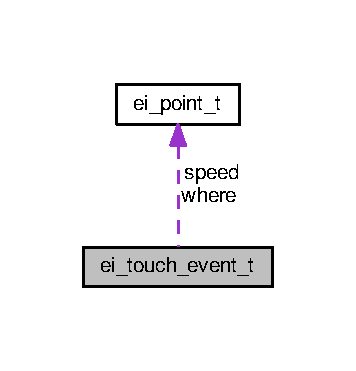
\includegraphics[width=171pt]{structei__touch__event__t__coll__graph}
\end{center}
\end{figure}
\subsection*{Public Attributes}
\begin{DoxyCompactItemize}
\item 
\hyperlink{structei__point__t}{ei\+\_\+point\+\_\+t} \hyperlink{structei__touch__event__t_a396ee9581e6e58e3462da797516ae928}{where}\hypertarget{structei__touch__event__t_a396ee9581e6e58e3462da797516ae928}{}\label{structei__touch__event__t_a396ee9581e6e58e3462da797516ae928}

\begin{DoxyCompactList}\small\item\em Where the touch was at the time of the event. \end{DoxyCompactList}\item 
\hyperlink{structei__point__t}{ei\+\_\+point\+\_\+t} \hyperlink{structei__touch__event__t_af155f4e0e04c9a97ec519e1dbd5b1422}{speed}\hypertarget{structei__touch__event__t_af155f4e0e04c9a97ec519e1dbd5b1422}{}\label{structei__touch__event__t_af155f4e0e04c9a97ec519e1dbd5b1422}

\begin{DoxyCompactList}\small\item\em Movement speed in pixels. \end{DoxyCompactList}\item 
int \hyperlink{structei__touch__event__t_a328a41ee9952d545b22c78047eaf09f6}{touch\+\_\+id}
\item 
\hyperlink{ei__types_8h_a383b9af13bd6a0a893096ead3c4d8e28}{ei\+\_\+bool\+\_\+t} \hyperlink{structei__touch__event__t_ad1ac5fff1b97acd2ef179412a753a517}{primary}
\begin{DoxyCompactList}\small\item\em it will stay the same for events from the same finger until the touch ends. \end{DoxyCompactList}\end{DoxyCompactItemize}


\subsection{Detailed Description}
The event parameter for mouse-\/related event types. 

\subsection{Member Data Documentation}
\index{ei\+\_\+touch\+\_\+event\+\_\+t@{ei\+\_\+touch\+\_\+event\+\_\+t}!primary@{primary}}
\index{primary@{primary}!ei\+\_\+touch\+\_\+event\+\_\+t@{ei\+\_\+touch\+\_\+event\+\_\+t}}
\subsubsection[{\texorpdfstring{primary}{primary}}]{\setlength{\rightskip}{0pt plus 5cm}{\bf ei\+\_\+bool\+\_\+t} ei\+\_\+touch\+\_\+event\+\_\+t\+::primary}\hypertarget{structei__touch__event__t_ad1ac5fff1b97acd2ef179412a753a517}{}\label{structei__touch__event__t_ad1ac5fff1b97acd2ef179412a753a517}


it will stay the same for events from the same finger until the touch ends. 

Whether this is the only/first touch or an additional touch. \index{ei\+\_\+touch\+\_\+event\+\_\+t@{ei\+\_\+touch\+\_\+event\+\_\+t}!touch\+\_\+id@{touch\+\_\+id}}
\index{touch\+\_\+id@{touch\+\_\+id}!ei\+\_\+touch\+\_\+event\+\_\+t@{ei\+\_\+touch\+\_\+event\+\_\+t}}
\subsubsection[{\texorpdfstring{touch\+\_\+id}{touch_id}}]{\setlength{\rightskip}{0pt plus 5cm}int ei\+\_\+touch\+\_\+event\+\_\+t\+::touch\+\_\+id}\hypertarget{structei__touch__event__t_a328a41ee9952d545b22c78047eaf09f6}{}\label{structei__touch__event__t_a328a41ee9952d545b22c78047eaf09f6}
An identifier for this touch. If supported by the device 

The documentation for this struct was generated from the following file\+:\begin{DoxyCompactItemize}
\item 
include/\hyperlink{ei__event_8h}{ei\+\_\+event.\+h}\end{DoxyCompactItemize}

\chapter{File Documentation}
\hypertarget{ei__event_8h}{}\section{include/ei\+\_\+event.h File Reference}
\label{ei__event_8h}\index{include/ei\+\_\+event.\+h@{include/ei\+\_\+event.\+h}}


Allows the binding and unbinding of callbacks to events.  


{\ttfamily \#include \char`\"{}ei\+\_\+types.\+h\char`\"{}}\\*
Include dependency graph for ei\+\_\+event.\+h\+:\nopagebreak
\begin{figure}[H]
\begin{center}
\leavevmode
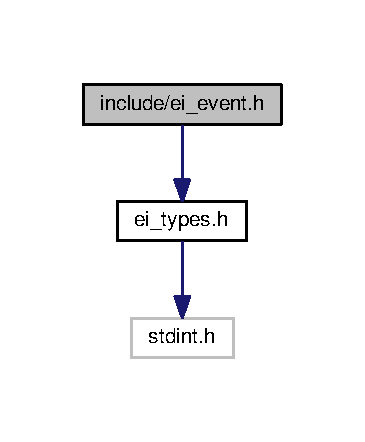
\includegraphics[width=175pt]{ei__event_8h__incl}
\end{center}
\end{figure}
\subsection*{Classes}
\begin{DoxyCompactItemize}
\item 
struct \hyperlink{structei__linked__tag__t}{ei\+\_\+linked\+\_\+tag\+\_\+t}
\begin{DoxyCompactList}\small\item\em A tag and a pointer to create a linked list. \end{DoxyCompactList}\item 
struct \hyperlink{structei__display__event__t}{ei\+\_\+display\+\_\+event\+\_\+t}
\begin{DoxyCompactList}\small\item\em The event parameter for display-\/related event types. \end{DoxyCompactList}\item 
struct \hyperlink{structei__key__event__t}{ei\+\_\+key\+\_\+event\+\_\+t}
\begin{DoxyCompactList}\small\item\em The event parameter for keyboard-\/related event types. \end{DoxyCompactList}\item 
struct \hyperlink{structei__mouse__event__t}{ei\+\_\+mouse\+\_\+event\+\_\+t}
\begin{DoxyCompactList}\small\item\em The event parameter for mouse-\/related event types. \end{DoxyCompactList}\item 
struct \hyperlink{structei__touch__event__t}{ei\+\_\+touch\+\_\+event\+\_\+t}
\begin{DoxyCompactList}\small\item\em The event parameter for mouse-\/related event types. \end{DoxyCompactList}\item 
struct \hyperlink{structei__app__event__t}{ei\+\_\+app\+\_\+event\+\_\+t}
\begin{DoxyCompactList}\small\item\em The event parameter for application defined event types. \end{DoxyCompactList}\item 
struct \hyperlink{structei__event__t}{ei\+\_\+event\+\_\+t}
\begin{DoxyCompactList}\small\item\em Describes an event. \end{DoxyCompactList}\end{DoxyCompactItemize}
\subsection*{Typedefs}
\begin{DoxyCompactItemize}
\item 
typedef char $\ast$ \hyperlink{ei__event_8h_a24a8242260cfd8ddb6ef915f3de5a10f}{ei\+\_\+tag\+\_\+t}\hypertarget{ei__event_8h_a24a8242260cfd8ddb6ef915f3de5a10f}{}\label{ei__event_8h_a24a8242260cfd8ddb6ef915f3de5a10f}

\begin{DoxyCompactList}\small\item\em A string that can be attached to a widget. All widget have the tag of the name of their widget class, and the tag \char`\"{}all\char`\"{}. \end{DoxyCompactList}\item 
typedef struct \hyperlink{structei__linked__tag__t}{ei\+\_\+linked\+\_\+tag\+\_\+t} \hyperlink{ei__event_8h_a1f068a6e43c1e260fafceca7d9f08960}{ei\+\_\+linked\+\_\+tag\+\_\+t}\hypertarget{ei__event_8h_a1f068a6e43c1e260fafceca7d9f08960}{}\label{ei__event_8h_a1f068a6e43c1e260fafceca7d9f08960}

\begin{DoxyCompactList}\small\item\em A tag and a pointer to create a linked list. \end{DoxyCompactList}\item 
typedef uint32\+\_\+t \hyperlink{ei__event_8h_abcdd2ef0f39179463f17a06be9bdf949}{ei\+\_\+modifier\+\_\+mask\+\_\+t}\hypertarget{ei__event_8h_abcdd2ef0f39179463f17a06be9bdf949}{}\label{ei__event_8h_abcdd2ef0f39179463f17a06be9bdf949}

\begin{DoxyCompactList}\small\item\em A bitfield indicating which of the modifier keys are currently pressed. \end{DoxyCompactList}\item 
typedef struct \hyperlink{structei__event__t}{ei\+\_\+event\+\_\+t} \hyperlink{ei__event_8h_a5fdf73bd9def856b6ea9edca6aa0423a}{ei\+\_\+event\+\_\+t}\hypertarget{ei__event_8h_a5fdf73bd9def856b6ea9edca6aa0423a}{}\label{ei__event_8h_a5fdf73bd9def856b6ea9edca6aa0423a}

\begin{DoxyCompactList}\small\item\em Describes an event. \end{DoxyCompactList}\end{DoxyCompactItemize}
\subsection*{Enumerations}
\begin{DoxyCompactItemize}
\item 
enum \hyperlink{ei__event_8h_a132dde064150d861ad24e9d839cbe007}{ei\+\_\+eventtype\+\_\+t} \{ \\*
\hyperlink{ei__event_8h_a132dde064150d861ad24e9d839cbe007a533f41177236ec3b01d8690765604d6c}{ei\+\_\+ev\+\_\+none} = 0, 
\hyperlink{ei__event_8h_a132dde064150d861ad24e9d839cbe007a429daab2361823f76417320fc66338d4}{ei\+\_\+ev\+\_\+app}, 
\hyperlink{ei__event_8h_a132dde064150d861ad24e9d839cbe007aeb7875975c5636463e26e87390f2fbf3}{ei\+\_\+ev\+\_\+display}, 
\hyperlink{ei__event_8h_a132dde064150d861ad24e9d839cbe007aa5fcf0b8e2fdda85acdde99bdd089cd3}{ei\+\_\+ev\+\_\+keydown}, 
\\*
\hyperlink{ei__event_8h_a132dde064150d861ad24e9d839cbe007af556498fd29604b3770b8fc2969cd3f1}{ei\+\_\+ev\+\_\+keyup}, 
\hyperlink{ei__event_8h_a132dde064150d861ad24e9d839cbe007a65746b5440ecd78bceecfaad7ee107ad}{ei\+\_\+ev\+\_\+keychar}, 
\hyperlink{ei__event_8h_a132dde064150d861ad24e9d839cbe007ae75b2b6a8423d54c46a418d222e0af66}{ei\+\_\+ev\+\_\+mouse\+\_\+buttondown}, 
\hyperlink{ei__event_8h_a132dde064150d861ad24e9d839cbe007aabd9931e36fb3628cc044a2aafc2c7e4}{ei\+\_\+ev\+\_\+mouse\+\_\+buttonup}, 
\\*
\hyperlink{ei__event_8h_a132dde064150d861ad24e9d839cbe007a5673338c91142f9c26826d1b52326b19}{ei\+\_\+ev\+\_\+mouse\+\_\+move}, 
\hyperlink{ei__event_8h_a132dde064150d861ad24e9d839cbe007ae79dd9ef27316f4cf4f6465883913e83}{ei\+\_\+ev\+\_\+touch\+\_\+begin}, 
\hyperlink{ei__event_8h_a132dde064150d861ad24e9d839cbe007ae9214f3221a0bc8aa9da20f1bb3f5d8e}{ei\+\_\+ev\+\_\+touch\+\_\+end}, 
\hyperlink{ei__event_8h_a132dde064150d861ad24e9d839cbe007af3c733a2ac0bb2442dc30f8e1c2ad9b4}{ei\+\_\+ev\+\_\+touch\+\_\+move}, 
\\*
\hyperlink{ei__event_8h_a132dde064150d861ad24e9d839cbe007a10fa93b6be568ea7175368c025506f6f}{ei\+\_\+ev\+\_\+last}
 \}\begin{DoxyCompactList}\small\item\em The types of events. \end{DoxyCompactList}
\item 
enum \hyperlink{ei__event_8h_a727655addb1c37c210f583964a1ac2b6}{ei\+\_\+modifier\+\_\+key\+\_\+t} \{ \\*
\hyperlink{ei__event_8h_a727655addb1c37c210f583964a1ac2b6a7daeb33b54ad2022a3fc709525617789}{ei\+\_\+mod\+\_\+shift} = 0x00001, 
\hyperlink{ei__event_8h_a727655addb1c37c210f583964a1ac2b6a4c074199e51f124821ee67357c7842b4}{ei\+\_\+mod\+\_\+ctrl} = 0x00002, 
\hyperlink{ei__event_8h_a727655addb1c37c210f583964a1ac2b6a16fa1ae2706337919c0562d8fbd40522}{ei\+\_\+mod\+\_\+alt} = 0x00004, 
\hyperlink{ei__event_8h_a727655addb1c37c210f583964a1ac2b6aabb5562f86439badd3cd94dc4e328640}{ei\+\_\+mod\+\_\+meta\+\_\+left} = 0x00008, 
\\*
\hyperlink{ei__event_8h_a727655addb1c37c210f583964a1ac2b6aa712981edbe0bac0bfc5c7bfaf2917c6}{ei\+\_\+mod\+\_\+meta\+\_\+right} = 0x00010, 
\hyperlink{ei__event_8h_a727655addb1c37c210f583964a1ac2b6ad916ab01279be9097ecf763adf325c5e}{ei\+\_\+mod\+\_\+alt\+\_\+grad} = 0x00040
 \}\begin{DoxyCompactList}\small\item\em The modifier keys (shift, alt, etc.) \end{DoxyCompactList}
\end{DoxyCompactItemize}


\subsection{Detailed Description}
Allows the binding and unbinding of callbacks to events. 

\begin{DoxyAuthor}{Author}
Created by François Bérard on 30.\+12.\+11. Copyright 2011 Ensimag. All rights reserved. 
\end{DoxyAuthor}


\subsection{Enumeration Type Documentation}
\index{ei\+\_\+event.\+h@{ei\+\_\+event.\+h}!ei\+\_\+eventtype\+\_\+t@{ei\+\_\+eventtype\+\_\+t}}
\index{ei\+\_\+eventtype\+\_\+t@{ei\+\_\+eventtype\+\_\+t}!ei\+\_\+event.\+h@{ei\+\_\+event.\+h}}
\subsubsection[{\texorpdfstring{ei\+\_\+eventtype\+\_\+t}{ei_eventtype_t}}]{\setlength{\rightskip}{0pt plus 5cm}enum {\bf ei\+\_\+eventtype\+\_\+t}}\hypertarget{ei__event_8h_a132dde064150d861ad24e9d839cbe007}{}\label{ei__event_8h_a132dde064150d861ad24e9d839cbe007}


The types of events. 

\begin{Desc}
\item[Enumerator]\par
\begin{description}
\index{ei\+\_\+ev\+\_\+none@{ei\+\_\+ev\+\_\+none}!ei\+\_\+event.\+h@{ei\+\_\+event.\+h}}\index{ei\+\_\+event.\+h@{ei\+\_\+event.\+h}!ei\+\_\+ev\+\_\+none@{ei\+\_\+ev\+\_\+none}}\item[{\em 
ei\+\_\+ev\+\_\+none\hypertarget{ei__event_8h_a132dde064150d861ad24e9d839cbe007a533f41177236ec3b01d8690765604d6c}{}\label{ei__event_8h_a132dde064150d861ad24e9d839cbe007a533f41177236ec3b01d8690765604d6c}
}]No event, used on an un-\/initialized structure. \index{ei\+\_\+ev\+\_\+app@{ei\+\_\+ev\+\_\+app}!ei\+\_\+event.\+h@{ei\+\_\+event.\+h}}\index{ei\+\_\+event.\+h@{ei\+\_\+event.\+h}!ei\+\_\+ev\+\_\+app@{ei\+\_\+ev\+\_\+app}}\item[{\em 
ei\+\_\+ev\+\_\+app\hypertarget{ei__event_8h_a132dde064150d861ad24e9d839cbe007a429daab2361823f76417320fc66338d4}{}\label{ei__event_8h_a132dde064150d861ad24e9d839cbe007a429daab2361823f76417320fc66338d4}
}]An application event, created by \hyperlink{hw__interface_8h_a1a1671a4990e4fa625693e8fe7536a1e}{hw\+\_\+event\+\_\+post\+\_\+app}. \index{ei\+\_\+ev\+\_\+display@{ei\+\_\+ev\+\_\+display}!ei\+\_\+event.\+h@{ei\+\_\+event.\+h}}\index{ei\+\_\+event.\+h@{ei\+\_\+event.\+h}!ei\+\_\+ev\+\_\+display@{ei\+\_\+ev\+\_\+display}}\item[{\em 
ei\+\_\+ev\+\_\+display\hypertarget{ei__event_8h_a132dde064150d861ad24e9d839cbe007aeb7875975c5636463e26e87390f2fbf3}{}\label{ei__event_8h_a132dde064150d861ad24e9d839cbe007aeb7875975c5636463e26e87390f2fbf3}
}]A display / window event. \index{ei\+\_\+ev\+\_\+keydown@{ei\+\_\+ev\+\_\+keydown}!ei\+\_\+event.\+h@{ei\+\_\+event.\+h}}\index{ei\+\_\+event.\+h@{ei\+\_\+event.\+h}!ei\+\_\+ev\+\_\+keydown@{ei\+\_\+ev\+\_\+keydown}}\item[{\em 
ei\+\_\+ev\+\_\+keydown\hypertarget{ei__event_8h_a132dde064150d861ad24e9d839cbe007aa5fcf0b8e2fdda85acdde99bdd089cd3}{}\label{ei__event_8h_a132dde064150d861ad24e9d839cbe007aa5fcf0b8e2fdda85acdde99bdd089cd3}
}]A keyboard key has been pressed. \index{ei\+\_\+ev\+\_\+keyup@{ei\+\_\+ev\+\_\+keyup}!ei\+\_\+event.\+h@{ei\+\_\+event.\+h}}\index{ei\+\_\+event.\+h@{ei\+\_\+event.\+h}!ei\+\_\+ev\+\_\+keyup@{ei\+\_\+ev\+\_\+keyup}}\item[{\em 
ei\+\_\+ev\+\_\+keyup\hypertarget{ei__event_8h_a132dde064150d861ad24e9d839cbe007af556498fd29604b3770b8fc2969cd3f1}{}\label{ei__event_8h_a132dde064150d861ad24e9d839cbe007af556498fd29604b3770b8fc2969cd3f1}
}]A keyboard key has been released. \index{ei\+\_\+ev\+\_\+keychar@{ei\+\_\+ev\+\_\+keychar}!ei\+\_\+event.\+h@{ei\+\_\+event.\+h}}\index{ei\+\_\+event.\+h@{ei\+\_\+event.\+h}!ei\+\_\+ev\+\_\+keychar@{ei\+\_\+ev\+\_\+keychar}}\item[{\em 
ei\+\_\+ev\+\_\+keychar\hypertarget{ei__event_8h_a132dde064150d861ad24e9d839cbe007a65746b5440ecd78bceecfaad7ee107ad}{}\label{ei__event_8h_a132dde064150d861ad24e9d839cbe007a65746b5440ecd78bceecfaad7ee107ad}
}]A character was typed on the keyboard. \index{ei\+\_\+ev\+\_\+mouse\+\_\+buttondown@{ei\+\_\+ev\+\_\+mouse\+\_\+buttondown}!ei\+\_\+event.\+h@{ei\+\_\+event.\+h}}\index{ei\+\_\+event.\+h@{ei\+\_\+event.\+h}!ei\+\_\+ev\+\_\+mouse\+\_\+buttondown@{ei\+\_\+ev\+\_\+mouse\+\_\+buttondown}}\item[{\em 
ei\+\_\+ev\+\_\+mouse\+\_\+buttondown\hypertarget{ei__event_8h_a132dde064150d861ad24e9d839cbe007ae75b2b6a8423d54c46a418d222e0af66}{}\label{ei__event_8h_a132dde064150d861ad24e9d839cbe007ae75b2b6a8423d54c46a418d222e0af66}
}]A mouse button has been pressed. \index{ei\+\_\+ev\+\_\+mouse\+\_\+buttonup@{ei\+\_\+ev\+\_\+mouse\+\_\+buttonup}!ei\+\_\+event.\+h@{ei\+\_\+event.\+h}}\index{ei\+\_\+event.\+h@{ei\+\_\+event.\+h}!ei\+\_\+ev\+\_\+mouse\+\_\+buttonup@{ei\+\_\+ev\+\_\+mouse\+\_\+buttonup}}\item[{\em 
ei\+\_\+ev\+\_\+mouse\+\_\+buttonup\hypertarget{ei__event_8h_a132dde064150d861ad24e9d839cbe007aabd9931e36fb3628cc044a2aafc2c7e4}{}\label{ei__event_8h_a132dde064150d861ad24e9d839cbe007aabd9931e36fb3628cc044a2aafc2c7e4}
}]A mouse button has been released. \index{ei\+\_\+ev\+\_\+mouse\+\_\+move@{ei\+\_\+ev\+\_\+mouse\+\_\+move}!ei\+\_\+event.\+h@{ei\+\_\+event.\+h}}\index{ei\+\_\+event.\+h@{ei\+\_\+event.\+h}!ei\+\_\+ev\+\_\+mouse\+\_\+move@{ei\+\_\+ev\+\_\+mouse\+\_\+move}}\item[{\em 
ei\+\_\+ev\+\_\+mouse\+\_\+move\hypertarget{ei__event_8h_a132dde064150d861ad24e9d839cbe007a5673338c91142f9c26826d1b52326b19}{}\label{ei__event_8h_a132dde064150d861ad24e9d839cbe007a5673338c91142f9c26826d1b52326b19}
}]The mouse has moved. \index{ei\+\_\+ev\+\_\+touch\+\_\+begin@{ei\+\_\+ev\+\_\+touch\+\_\+begin}!ei\+\_\+event.\+h@{ei\+\_\+event.\+h}}\index{ei\+\_\+event.\+h@{ei\+\_\+event.\+h}!ei\+\_\+ev\+\_\+touch\+\_\+begin@{ei\+\_\+ev\+\_\+touch\+\_\+begin}}\item[{\em 
ei\+\_\+ev\+\_\+touch\+\_\+begin\hypertarget{ei__event_8h_a132dde064150d861ad24e9d839cbe007ae79dd9ef27316f4cf4f6465883913e83}{}\label{ei__event_8h_a132dde064150d861ad24e9d839cbe007ae79dd9ef27316f4cf4f6465883913e83}
}]The touch input device registered a new touch. \index{ei\+\_\+ev\+\_\+touch\+\_\+end@{ei\+\_\+ev\+\_\+touch\+\_\+end}!ei\+\_\+event.\+h@{ei\+\_\+event.\+h}}\index{ei\+\_\+event.\+h@{ei\+\_\+event.\+h}!ei\+\_\+ev\+\_\+touch\+\_\+end@{ei\+\_\+ev\+\_\+touch\+\_\+end}}\item[{\em 
ei\+\_\+ev\+\_\+touch\+\_\+end\hypertarget{ei__event_8h_a132dde064150d861ad24e9d839cbe007ae9214f3221a0bc8aa9da20f1bb3f5d8e}{}\label{ei__event_8h_a132dde064150d861ad24e9d839cbe007ae9214f3221a0bc8aa9da20f1bb3f5d8e}
}]A touch ended. \index{ei\+\_\+ev\+\_\+touch\+\_\+move@{ei\+\_\+ev\+\_\+touch\+\_\+move}!ei\+\_\+event.\+h@{ei\+\_\+event.\+h}}\index{ei\+\_\+event.\+h@{ei\+\_\+event.\+h}!ei\+\_\+ev\+\_\+touch\+\_\+move@{ei\+\_\+ev\+\_\+touch\+\_\+move}}\item[{\em 
ei\+\_\+ev\+\_\+touch\+\_\+move\hypertarget{ei__event_8h_a132dde064150d861ad24e9d839cbe007af3c733a2ac0bb2442dc30f8e1c2ad9b4}{}\label{ei__event_8h_a132dde064150d861ad24e9d839cbe007af3c733a2ac0bb2442dc30f8e1c2ad9b4}
}]The position of a touch changed. \index{ei\+\_\+ev\+\_\+last@{ei\+\_\+ev\+\_\+last}!ei\+\_\+event.\+h@{ei\+\_\+event.\+h}}\index{ei\+\_\+event.\+h@{ei\+\_\+event.\+h}!ei\+\_\+ev\+\_\+last@{ei\+\_\+ev\+\_\+last}}\item[{\em 
ei\+\_\+ev\+\_\+last\hypertarget{ei__event_8h_a132dde064150d861ad24e9d839cbe007a10fa93b6be568ea7175368c025506f6f}{}\label{ei__event_8h_a132dde064150d861ad24e9d839cbe007a10fa93b6be568ea7175368c025506f6f}
}]Last event type, its value is the number of event types. \end{description}
\end{Desc}
\index{ei\+\_\+event.\+h@{ei\+\_\+event.\+h}!ei\+\_\+modifier\+\_\+key\+\_\+t@{ei\+\_\+modifier\+\_\+key\+\_\+t}}
\index{ei\+\_\+modifier\+\_\+key\+\_\+t@{ei\+\_\+modifier\+\_\+key\+\_\+t}!ei\+\_\+event.\+h@{ei\+\_\+event.\+h}}
\subsubsection[{\texorpdfstring{ei\+\_\+modifier\+\_\+key\+\_\+t}{ei_modifier_key_t}}]{\setlength{\rightskip}{0pt plus 5cm}enum {\bf ei\+\_\+modifier\+\_\+key\+\_\+t}}\hypertarget{ei__event_8h_a727655addb1c37c210f583964a1ac2b6}{}\label{ei__event_8h_a727655addb1c37c210f583964a1ac2b6}


The modifier keys (shift, alt, etc.) 

\begin{Desc}
\item[Enumerator]\par
\begin{description}
\index{ei\+\_\+mod\+\_\+shift@{ei\+\_\+mod\+\_\+shift}!ei\+\_\+event.\+h@{ei\+\_\+event.\+h}}\index{ei\+\_\+event.\+h@{ei\+\_\+event.\+h}!ei\+\_\+mod\+\_\+shift@{ei\+\_\+mod\+\_\+shift}}\item[{\em 
ei\+\_\+mod\+\_\+shift\hypertarget{ei__event_8h_a727655addb1c37c210f583964a1ac2b6a7daeb33b54ad2022a3fc709525617789}{}\label{ei__event_8h_a727655addb1c37c210f583964a1ac2b6a7daeb33b54ad2022a3fc709525617789}
}]The \char`\"{}shift\char`\"{} key. \index{ei\+\_\+mod\+\_\+ctrl@{ei\+\_\+mod\+\_\+ctrl}!ei\+\_\+event.\+h@{ei\+\_\+event.\+h}}\index{ei\+\_\+event.\+h@{ei\+\_\+event.\+h}!ei\+\_\+mod\+\_\+ctrl@{ei\+\_\+mod\+\_\+ctrl}}\item[{\em 
ei\+\_\+mod\+\_\+ctrl\hypertarget{ei__event_8h_a727655addb1c37c210f583964a1ac2b6a4c074199e51f124821ee67357c7842b4}{}\label{ei__event_8h_a727655addb1c37c210f583964a1ac2b6a4c074199e51f124821ee67357c7842b4}
}]The \char`\"{}control\char`\"{} key. \index{ei\+\_\+mod\+\_\+alt@{ei\+\_\+mod\+\_\+alt}!ei\+\_\+event.\+h@{ei\+\_\+event.\+h}}\index{ei\+\_\+event.\+h@{ei\+\_\+event.\+h}!ei\+\_\+mod\+\_\+alt@{ei\+\_\+mod\+\_\+alt}}\item[{\em 
ei\+\_\+mod\+\_\+alt\hypertarget{ei__event_8h_a727655addb1c37c210f583964a1ac2b6a16fa1ae2706337919c0562d8fbd40522}{}\label{ei__event_8h_a727655addb1c37c210f583964a1ac2b6a16fa1ae2706337919c0562d8fbd40522}
}]The \char`\"{}alternate\char`\"{} key at the left of the space bar. \index{ei\+\_\+mod\+\_\+meta\+\_\+left@{ei\+\_\+mod\+\_\+meta\+\_\+left}!ei\+\_\+event.\+h@{ei\+\_\+event.\+h}}\index{ei\+\_\+event.\+h@{ei\+\_\+event.\+h}!ei\+\_\+mod\+\_\+meta\+\_\+left@{ei\+\_\+mod\+\_\+meta\+\_\+left}}\item[{\em 
ei\+\_\+mod\+\_\+meta\+\_\+left\hypertarget{ei__event_8h_a727655addb1c37c210f583964a1ac2b6aabb5562f86439badd3cd94dc4e328640}{}\label{ei__event_8h_a727655addb1c37c210f583964a1ac2b6aabb5562f86439badd3cd94dc4e328640}
}]The \char`\"{}meta\char`\"{} (command) key at the left of the space bar. \index{ei\+\_\+mod\+\_\+meta\+\_\+right@{ei\+\_\+mod\+\_\+meta\+\_\+right}!ei\+\_\+event.\+h@{ei\+\_\+event.\+h}}\index{ei\+\_\+event.\+h@{ei\+\_\+event.\+h}!ei\+\_\+mod\+\_\+meta\+\_\+right@{ei\+\_\+mod\+\_\+meta\+\_\+right}}\item[{\em 
ei\+\_\+mod\+\_\+meta\+\_\+right\hypertarget{ei__event_8h_a727655addb1c37c210f583964a1ac2b6aa712981edbe0bac0bfc5c7bfaf2917c6}{}\label{ei__event_8h_a727655addb1c37c210f583964a1ac2b6aa712981edbe0bac0bfc5c7bfaf2917c6}
}]The \char`\"{}meta\char`\"{} (command) key at the right of the space bar. \index{ei\+\_\+mod\+\_\+alt\+\_\+grad@{ei\+\_\+mod\+\_\+alt\+\_\+grad}!ei\+\_\+event.\+h@{ei\+\_\+event.\+h}}\index{ei\+\_\+event.\+h@{ei\+\_\+event.\+h}!ei\+\_\+mod\+\_\+alt\+\_\+grad@{ei\+\_\+mod\+\_\+alt\+\_\+grad}}\item[{\em 
ei\+\_\+mod\+\_\+alt\+\_\+grad\hypertarget{ei__event_8h_a727655addb1c37c210f583964a1ac2b6ad916ab01279be9097ecf763adf325c5e}{}\label{ei__event_8h_a727655addb1c37c210f583964a1ac2b6ad916ab01279be9097ecf763adf325c5e}
}]The \char`\"{}alternate\char`\"{} key at the right of the space bar. \end{description}
\end{Desc}

\hypertarget{ei__main_8h}{}\section{include/ei\+\_\+main.h File Reference}
\label{ei__main_8h}\index{include/ei\+\_\+main.\+h@{include/ei\+\_\+main.\+h}}


Declares the \char`\"{}ei\+\_\+main\char`\"{} function\+: the main function of programs built with the libei.  


\subsection*{Functions}
\begin{DoxyCompactItemize}
\item 
int \hyperlink{ei__main_8h_a439ac1da07a00a0abff8d762e562c4ec}{ei\+\_\+main} (int argc, char $\ast$argv\mbox{[}$\,$\mbox{]})
\begin{DoxyCompactList}\small\item\em The main function of the program. \end{DoxyCompactList}\end{DoxyCompactItemize}


\subsection{Detailed Description}
Declares the \char`\"{}ei\+\_\+main\char`\"{} function\+: the main function of programs built with the libei. 

\begin{DoxyAuthor}{Author}
Created by François Bérard on 30.\+12.\+11. Copyright 2011 Ensimag. All rights reserved. 
\end{DoxyAuthor}


\subsection{Function Documentation}
\index{ei\+\_\+main.\+h@{ei\+\_\+main.\+h}!ei\+\_\+main@{ei\+\_\+main}}
\index{ei\+\_\+main@{ei\+\_\+main}!ei\+\_\+main.\+h@{ei\+\_\+main.\+h}}
\subsubsection[{\texorpdfstring{ei\+\_\+main(int argc, char $\ast$argv[])}{ei_main(int argc, char *argv[])}}]{\setlength{\rightskip}{0pt plus 5cm}int ei\+\_\+main (
\begin{DoxyParamCaption}
\item[{int}]{argc, }
\item[{char $\ast$}]{argv\mbox{[}$\,$\mbox{]}}
\end{DoxyParamCaption}
)}\hypertarget{ei__main_8h_a439ac1da07a00a0abff8d762e562c4ec}{}\label{ei__main_8h_a439ac1da07a00a0abff8d762e562c4ec}


The main function of the program. 

Programmers must not define their main function in a function called \char`\"{}main\char`\"{}, because the \char`\"{}main\char`\"{} function is defined by S\+DL and linked with in the libeibase library.


\begin{DoxyParams}{Parameters}
{\em argc,argv} & The parameters that were passed the the \char`\"{}main\char`\"{} function.\\
\hline
\end{DoxyParams}
\begin{DoxyReturn}{Returns}
An error code\+: 0 means ok, 1 means error. 
\end{DoxyReturn}

\hypertarget{ei__types_8h}{}\section{include/ei\+\_\+types.h File Reference}
\label{ei__types_8h}\index{include/ei\+\_\+types.\+h@{include/ei\+\_\+types.\+h}}


Type, constant, and global definitions for the ei library.  


{\ttfamily \#include $<$stdint.\+h$>$}\\*
Include dependency graph for ei\+\_\+types.\+h\+:
\nopagebreak
\begin{figure}[H]
\begin{center}
\leavevmode
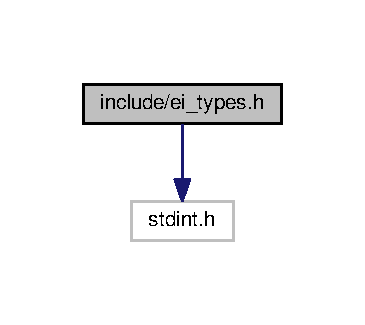
\includegraphics[width=175pt]{ei__types_8h__incl}
\end{center}
\end{figure}
This graph shows which files directly or indirectly include this file\+:
\nopagebreak
\begin{figure}[H]
\begin{center}
\leavevmode
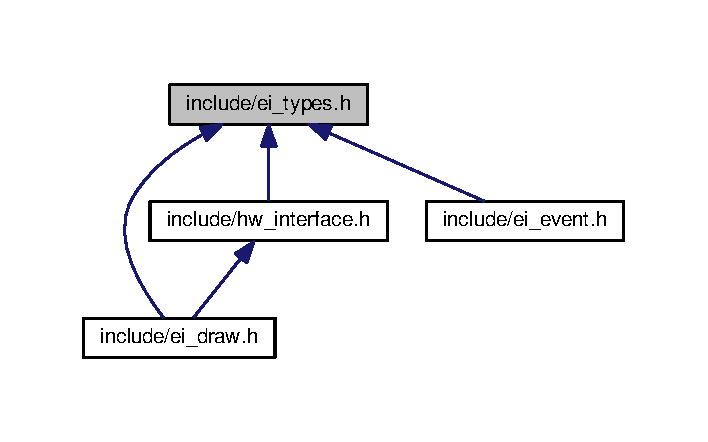
\includegraphics[width=308pt]{ei__types_8h__dep__incl}
\end{center}
\end{figure}
\subsection*{Classes}
\begin{DoxyCompactItemize}
\item 
struct \hyperlink{structei__point__t}{ei\+\_\+point\+\_\+t}
\begin{DoxyCompactList}\small\item\em A 2-\/D point with integer coordinates. \end{DoxyCompactList}\item 
struct \hyperlink{structei__size__t}{ei\+\_\+size\+\_\+t}
\begin{DoxyCompactList}\small\item\em A 2-\/D size with integer dimensions. \end{DoxyCompactList}\item 
struct \hyperlink{structei__rect__t}{ei\+\_\+rect\+\_\+t}
\begin{DoxyCompactList}\small\item\em A rectangle defined by its top-\/left corner, and its size. \end{DoxyCompactList}\item 
struct \hyperlink{structei__linked__rect__t}{ei\+\_\+linked\+\_\+rect\+\_\+t}
\begin{DoxyCompactList}\small\item\em A rectangle plus a pointer to create a linked list. \end{DoxyCompactList}\item 
struct \hyperlink{structei__linked__point__t}{ei\+\_\+linked\+\_\+point\+\_\+t}
\begin{DoxyCompactList}\small\item\em A point plus a pointer to create a linked list. \end{DoxyCompactList}\item 
struct \hyperlink{structei__color__t}{ei\+\_\+color\+\_\+t}
\begin{DoxyCompactList}\small\item\em A color with transparency. \end{DoxyCompactList}\end{DoxyCompactItemize}
\subsection*{Typedefs}
\begin{DoxyCompactItemize}
\item 
typedef struct \hyperlink{structei__linked__rect__t}{ei\+\_\+linked\+\_\+rect\+\_\+t} \hyperlink{ei__types_8h_a16241a27b7fb48452a6386e58494cc9a}{ei\+\_\+linked\+\_\+rect\+\_\+t}\hypertarget{ei__types_8h_a16241a27b7fb48452a6386e58494cc9a}{}\label{ei__types_8h_a16241a27b7fb48452a6386e58494cc9a}

\begin{DoxyCompactList}\small\item\em A rectangle plus a pointer to create a linked list. \end{DoxyCompactList}\item 
typedef struct \hyperlink{structei__linked__point__t}{ei\+\_\+linked\+\_\+point\+\_\+t} \hyperlink{ei__types_8h_aaa3f2e86217750f9c3c734bde1ffa41f}{ei\+\_\+linked\+\_\+point\+\_\+t}\hypertarget{ei__types_8h_aaa3f2e86217750f9c3c734bde1ffa41f}{}\label{ei__types_8h_aaa3f2e86217750f9c3c734bde1ffa41f}

\begin{DoxyCompactList}\small\item\em A point plus a pointer to create a linked list. \end{DoxyCompactList}\item 
typedef void $\ast$ \hyperlink{ei__types_8h_a22c8198e4d641e4bc67bb17f9c6bcda7}{ei\+\_\+font\+\_\+t}
\begin{DoxyCompactList}\small\item\em An opaque type for handling fonts. \end{DoxyCompactList}\end{DoxyCompactItemize}
\subsection*{Enumerations}
\begin{DoxyCompactItemize}
\item 
enum \hyperlink{ei__types_8h_a383b9af13bd6a0a893096ead3c4d8e28}{ei\+\_\+bool\+\_\+t} \{ {\bfseries E\+I\+\_\+\+F\+A\+L\+SE} = 0, 
{\bfseries E\+I\+\_\+\+T\+R\+UE} = 1
 \}\hypertarget{ei__types_8h_a383b9af13bd6a0a893096ead3c4d8e28}{}\label{ei__types_8h_a383b9af13bd6a0a893096ead3c4d8e28}
\begin{DoxyCompactList}\small\item\em The boolean type used in the library. \end{DoxyCompactList}
\item 
enum \hyperlink{ei__types_8h_a3852c963af609d31d7cfcff79c4c8450}{ei\+\_\+anchor\+\_\+t} \{ \\*
\hyperlink{ei__types_8h_a3852c963af609d31d7cfcff79c4c8450a00688941d6793b4165bbc56edb70646a}{ei\+\_\+anc\+\_\+none} = 0, 
\hyperlink{ei__types_8h_a3852c963af609d31d7cfcff79c4c8450a5704b2469014b3e93fbdb0b297ed92b0}{ei\+\_\+anc\+\_\+center}, 
\hyperlink{ei__types_8h_a3852c963af609d31d7cfcff79c4c8450abb9d5dcbb25572cab716280dbe72014d}{ei\+\_\+anc\+\_\+north}, 
\hyperlink{ei__types_8h_a3852c963af609d31d7cfcff79c4c8450af4ba72d1581a2e133eaeb6c00c912cff}{ei\+\_\+anc\+\_\+northeast}, 
\\*
\hyperlink{ei__types_8h_a3852c963af609d31d7cfcff79c4c8450ac60193e3f00916df2272dee7b33c1143}{ei\+\_\+anc\+\_\+east}, 
\hyperlink{ei__types_8h_a3852c963af609d31d7cfcff79c4c8450ac6ab86aaa5a6f70cf4a49ed317686c7e}{ei\+\_\+anc\+\_\+southeast}, 
\hyperlink{ei__types_8h_a3852c963af609d31d7cfcff79c4c8450a912ba0dd51dde60a610fbce211cf1b35}{ei\+\_\+anc\+\_\+south}, 
\hyperlink{ei__types_8h_a3852c963af609d31d7cfcff79c4c8450a200959a22ba17a83310a97570f62f392}{ei\+\_\+anc\+\_\+southwest}, 
\\*
\hyperlink{ei__types_8h_a3852c963af609d31d7cfcff79c4c8450af260d86ff3940d57139f0f8de9488512}{ei\+\_\+anc\+\_\+west}, 
\hyperlink{ei__types_8h_a3852c963af609d31d7cfcff79c4c8450a696c63e5bb8cab534cdf59d9a97f836b}{ei\+\_\+anc\+\_\+northwest}
 \}\begin{DoxyCompactList}\small\item\em Identifies one particular point of a rectangle. \end{DoxyCompactList}
\item 
enum \hyperlink{ei__types_8h_aa79a32b1d8ece0e44cfa394e870b270b}{ei\+\_\+relief\+\_\+t} \{ \hyperlink{ei__types_8h_aa79a32b1d8ece0e44cfa394e870b270ba105222bc995071e84bce027c90a59b62}{ei\+\_\+relief\+\_\+none} = 0, 
\hyperlink{ei__types_8h_aa79a32b1d8ece0e44cfa394e870b270bac1e7867185743599ffcceb42784bd4e3}{ei\+\_\+relief\+\_\+raised}, 
\hyperlink{ei__types_8h_aa79a32b1d8ece0e44cfa394e870b270ba227a7ad58efd20f955450357c0bd4b36}{ei\+\_\+relief\+\_\+sunken}
 \}\begin{DoxyCompactList}\small\item\em Type of relief. \end{DoxyCompactList}
\item 
enum \hyperlink{ei__types_8h_ab5d9ff46ba9b2c9fa6d6fbd2594c6439}{ei\+\_\+axis\+\_\+set\+\_\+t} \{ \hyperlink{ei__types_8h_ab5d9ff46ba9b2c9fa6d6fbd2594c6439ae34dee3f21cd76dae607d8334d3bab50}{ei\+\_\+axis\+\_\+none} = 0, 
\hyperlink{ei__types_8h_ab5d9ff46ba9b2c9fa6d6fbd2594c6439a7a26f78919e1c485e2270b9f5a7271bf}{ei\+\_\+axis\+\_\+x}, 
\hyperlink{ei__types_8h_ab5d9ff46ba9b2c9fa6d6fbd2594c6439af3316aa4c9c58d8e451a9a1c8a72e38d}{ei\+\_\+axis\+\_\+y}, 
\hyperlink{ei__types_8h_ab5d9ff46ba9b2c9fa6d6fbd2594c6439a6e6ffa2a8d854858429d6f54d94919a9}{ei\+\_\+axis\+\_\+both}
 \}\begin{DoxyCompactList}\small\item\em Set of axis. \end{DoxyCompactList}
\end{DoxyCompactItemize}
\subsection*{Variables}
\begin{DoxyCompactItemize}
\item 
\hyperlink{ei__types_8h_a22c8198e4d641e4bc67bb17f9c6bcda7}{ei\+\_\+font\+\_\+t} \hyperlink{ei__types_8h_a722bfa1a8a9a4202fb2d4abce2f06a8c}{ei\+\_\+default\+\_\+font}\hypertarget{ei__types_8h_a722bfa1a8a9a4202fb2d4abce2f06a8c}{}\label{ei__types_8h_a722bfa1a8a9a4202fb2d4abce2f06a8c}

\begin{DoxyCompactList}\small\item\em The default font used in widgets. \end{DoxyCompactList}\end{DoxyCompactItemize}


\subsection{Detailed Description}
Type, constant, and global definitions for the ei library. 

Created by François Bérard on 18.\+12.\+11. Copyright 2011 Ensimag. All rights reserved. 

\subsection{Typedef Documentation}
\index{ei\+\_\+types.\+h@{ei\+\_\+types.\+h}!ei\+\_\+font\+\_\+t@{ei\+\_\+font\+\_\+t}}
\index{ei\+\_\+font\+\_\+t@{ei\+\_\+font\+\_\+t}!ei\+\_\+types.\+h@{ei\+\_\+types.\+h}}
\subsubsection[{\texorpdfstring{ei\+\_\+font\+\_\+t}{ei_font_t}}]{\setlength{\rightskip}{0pt plus 5cm}typedef void$\ast$ {\bf ei\+\_\+font\+\_\+t}}\hypertarget{ei__types_8h_a22c8198e4d641e4bc67bb17f9c6bcda7}{}\label{ei__types_8h_a22c8198e4d641e4bc67bb17f9c6bcda7}


An opaque type for handling fonts. 

Fonts are created by calling \hyperlink{hw__interface_8h_a9c6b86bcbcdd0b3e590e1e33fcf893d7}{hw\+\_\+text\+\_\+font\+\_\+create} and released by calling \hyperlink{hw__interface_8h_a2ac46d37db4c40adc10e3afb137f9f02}{hw\+\_\+text\+\_\+font\+\_\+free}. 

\subsection{Enumeration Type Documentation}
\index{ei\+\_\+types.\+h@{ei\+\_\+types.\+h}!ei\+\_\+anchor\+\_\+t@{ei\+\_\+anchor\+\_\+t}}
\index{ei\+\_\+anchor\+\_\+t@{ei\+\_\+anchor\+\_\+t}!ei\+\_\+types.\+h@{ei\+\_\+types.\+h}}
\subsubsection[{\texorpdfstring{ei\+\_\+anchor\+\_\+t}{ei_anchor_t}}]{\setlength{\rightskip}{0pt plus 5cm}enum {\bf ei\+\_\+anchor\+\_\+t}}\hypertarget{ei__types_8h_a3852c963af609d31d7cfcff79c4c8450}{}\label{ei__types_8h_a3852c963af609d31d7cfcff79c4c8450}


Identifies one particular point of a rectangle. 

\begin{Desc}
\item[Enumerator]\par
\begin{description}
\index{ei\+\_\+anc\+\_\+none@{ei\+\_\+anc\+\_\+none}!ei\+\_\+types.\+h@{ei\+\_\+types.\+h}}\index{ei\+\_\+types.\+h@{ei\+\_\+types.\+h}!ei\+\_\+anc\+\_\+none@{ei\+\_\+anc\+\_\+none}}\item[{\em 
ei\+\_\+anc\+\_\+none\hypertarget{ei__types_8h_a3852c963af609d31d7cfcff79c4c8450a00688941d6793b4165bbc56edb70646a}{}\label{ei__types_8h_a3852c963af609d31d7cfcff79c4c8450a00688941d6793b4165bbc56edb70646a}
}]No anchor defined. \index{ei\+\_\+anc\+\_\+center@{ei\+\_\+anc\+\_\+center}!ei\+\_\+types.\+h@{ei\+\_\+types.\+h}}\index{ei\+\_\+types.\+h@{ei\+\_\+types.\+h}!ei\+\_\+anc\+\_\+center@{ei\+\_\+anc\+\_\+center}}\item[{\em 
ei\+\_\+anc\+\_\+center\hypertarget{ei__types_8h_a3852c963af609d31d7cfcff79c4c8450a5704b2469014b3e93fbdb0b297ed92b0}{}\label{ei__types_8h_a3852c963af609d31d7cfcff79c4c8450a5704b2469014b3e93fbdb0b297ed92b0}
}]Anchor in the center. \index{ei\+\_\+anc\+\_\+north@{ei\+\_\+anc\+\_\+north}!ei\+\_\+types.\+h@{ei\+\_\+types.\+h}}\index{ei\+\_\+types.\+h@{ei\+\_\+types.\+h}!ei\+\_\+anc\+\_\+north@{ei\+\_\+anc\+\_\+north}}\item[{\em 
ei\+\_\+anc\+\_\+north\hypertarget{ei__types_8h_a3852c963af609d31d7cfcff79c4c8450abb9d5dcbb25572cab716280dbe72014d}{}\label{ei__types_8h_a3852c963af609d31d7cfcff79c4c8450abb9d5dcbb25572cab716280dbe72014d}
}]Anchor on the top side, centered horizontally. \index{ei\+\_\+anc\+\_\+northeast@{ei\+\_\+anc\+\_\+northeast}!ei\+\_\+types.\+h@{ei\+\_\+types.\+h}}\index{ei\+\_\+types.\+h@{ei\+\_\+types.\+h}!ei\+\_\+anc\+\_\+northeast@{ei\+\_\+anc\+\_\+northeast}}\item[{\em 
ei\+\_\+anc\+\_\+northeast\hypertarget{ei__types_8h_a3852c963af609d31d7cfcff79c4c8450af4ba72d1581a2e133eaeb6c00c912cff}{}\label{ei__types_8h_a3852c963af609d31d7cfcff79c4c8450af4ba72d1581a2e133eaeb6c00c912cff}
}]Anchor on the top-\/right corner. \index{ei\+\_\+anc\+\_\+east@{ei\+\_\+anc\+\_\+east}!ei\+\_\+types.\+h@{ei\+\_\+types.\+h}}\index{ei\+\_\+types.\+h@{ei\+\_\+types.\+h}!ei\+\_\+anc\+\_\+east@{ei\+\_\+anc\+\_\+east}}\item[{\em 
ei\+\_\+anc\+\_\+east\hypertarget{ei__types_8h_a3852c963af609d31d7cfcff79c4c8450ac60193e3f00916df2272dee7b33c1143}{}\label{ei__types_8h_a3852c963af609d31d7cfcff79c4c8450ac60193e3f00916df2272dee7b33c1143}
}]Anchor on the right side, centered vertically. \index{ei\+\_\+anc\+\_\+southeast@{ei\+\_\+anc\+\_\+southeast}!ei\+\_\+types.\+h@{ei\+\_\+types.\+h}}\index{ei\+\_\+types.\+h@{ei\+\_\+types.\+h}!ei\+\_\+anc\+\_\+southeast@{ei\+\_\+anc\+\_\+southeast}}\item[{\em 
ei\+\_\+anc\+\_\+southeast\hypertarget{ei__types_8h_a3852c963af609d31d7cfcff79c4c8450ac6ab86aaa5a6f70cf4a49ed317686c7e}{}\label{ei__types_8h_a3852c963af609d31d7cfcff79c4c8450ac6ab86aaa5a6f70cf4a49ed317686c7e}
}]Anchor on the bottom-\/right corner. \index{ei\+\_\+anc\+\_\+south@{ei\+\_\+anc\+\_\+south}!ei\+\_\+types.\+h@{ei\+\_\+types.\+h}}\index{ei\+\_\+types.\+h@{ei\+\_\+types.\+h}!ei\+\_\+anc\+\_\+south@{ei\+\_\+anc\+\_\+south}}\item[{\em 
ei\+\_\+anc\+\_\+south\hypertarget{ei__types_8h_a3852c963af609d31d7cfcff79c4c8450a912ba0dd51dde60a610fbce211cf1b35}{}\label{ei__types_8h_a3852c963af609d31d7cfcff79c4c8450a912ba0dd51dde60a610fbce211cf1b35}
}]Anchor on the bottom side, centered horizontally. \index{ei\+\_\+anc\+\_\+southwest@{ei\+\_\+anc\+\_\+southwest}!ei\+\_\+types.\+h@{ei\+\_\+types.\+h}}\index{ei\+\_\+types.\+h@{ei\+\_\+types.\+h}!ei\+\_\+anc\+\_\+southwest@{ei\+\_\+anc\+\_\+southwest}}\item[{\em 
ei\+\_\+anc\+\_\+southwest\hypertarget{ei__types_8h_a3852c963af609d31d7cfcff79c4c8450a200959a22ba17a83310a97570f62f392}{}\label{ei__types_8h_a3852c963af609d31d7cfcff79c4c8450a200959a22ba17a83310a97570f62f392}
}]Anchor on the bottom-\/left corner. \index{ei\+\_\+anc\+\_\+west@{ei\+\_\+anc\+\_\+west}!ei\+\_\+types.\+h@{ei\+\_\+types.\+h}}\index{ei\+\_\+types.\+h@{ei\+\_\+types.\+h}!ei\+\_\+anc\+\_\+west@{ei\+\_\+anc\+\_\+west}}\item[{\em 
ei\+\_\+anc\+\_\+west\hypertarget{ei__types_8h_a3852c963af609d31d7cfcff79c4c8450af260d86ff3940d57139f0f8de9488512}{}\label{ei__types_8h_a3852c963af609d31d7cfcff79c4c8450af260d86ff3940d57139f0f8de9488512}
}]Anchor on the left side, centered vertically. \index{ei\+\_\+anc\+\_\+northwest@{ei\+\_\+anc\+\_\+northwest}!ei\+\_\+types.\+h@{ei\+\_\+types.\+h}}\index{ei\+\_\+types.\+h@{ei\+\_\+types.\+h}!ei\+\_\+anc\+\_\+northwest@{ei\+\_\+anc\+\_\+northwest}}\item[{\em 
ei\+\_\+anc\+\_\+northwest\hypertarget{ei__types_8h_a3852c963af609d31d7cfcff79c4c8450a696c63e5bb8cab534cdf59d9a97f836b}{}\label{ei__types_8h_a3852c963af609d31d7cfcff79c4c8450a696c63e5bb8cab534cdf59d9a97f836b}
}]Anchor on the top-\/left corner. \end{description}
\end{Desc}
\index{ei\+\_\+types.\+h@{ei\+\_\+types.\+h}!ei\+\_\+axis\+\_\+set\+\_\+t@{ei\+\_\+axis\+\_\+set\+\_\+t}}
\index{ei\+\_\+axis\+\_\+set\+\_\+t@{ei\+\_\+axis\+\_\+set\+\_\+t}!ei\+\_\+types.\+h@{ei\+\_\+types.\+h}}
\subsubsection[{\texorpdfstring{ei\+\_\+axis\+\_\+set\+\_\+t}{ei_axis_set_t}}]{\setlength{\rightskip}{0pt plus 5cm}enum {\bf ei\+\_\+axis\+\_\+set\+\_\+t}}\hypertarget{ei__types_8h_ab5d9ff46ba9b2c9fa6d6fbd2594c6439}{}\label{ei__types_8h_ab5d9ff46ba9b2c9fa6d6fbd2594c6439}


Set of axis. 

\begin{Desc}
\item[Enumerator]\par
\begin{description}
\index{ei\+\_\+axis\+\_\+none@{ei\+\_\+axis\+\_\+none}!ei\+\_\+types.\+h@{ei\+\_\+types.\+h}}\index{ei\+\_\+types.\+h@{ei\+\_\+types.\+h}!ei\+\_\+axis\+\_\+none@{ei\+\_\+axis\+\_\+none}}\item[{\em 
ei\+\_\+axis\+\_\+none\hypertarget{ei__types_8h_ab5d9ff46ba9b2c9fa6d6fbd2594c6439ae34dee3f21cd76dae607d8334d3bab50}{}\label{ei__types_8h_ab5d9ff46ba9b2c9fa6d6fbd2594c6439ae34dee3f21cd76dae607d8334d3bab50}
}]No axis. \index{ei\+\_\+axis\+\_\+x@{ei\+\_\+axis\+\_\+x}!ei\+\_\+types.\+h@{ei\+\_\+types.\+h}}\index{ei\+\_\+types.\+h@{ei\+\_\+types.\+h}!ei\+\_\+axis\+\_\+x@{ei\+\_\+axis\+\_\+x}}\item[{\em 
ei\+\_\+axis\+\_\+x\hypertarget{ei__types_8h_ab5d9ff46ba9b2c9fa6d6fbd2594c6439a7a26f78919e1c485e2270b9f5a7271bf}{}\label{ei__types_8h_ab5d9ff46ba9b2c9fa6d6fbd2594c6439a7a26f78919e1c485e2270b9f5a7271bf}
}]Horizontal axis. \index{ei\+\_\+axis\+\_\+y@{ei\+\_\+axis\+\_\+y}!ei\+\_\+types.\+h@{ei\+\_\+types.\+h}}\index{ei\+\_\+types.\+h@{ei\+\_\+types.\+h}!ei\+\_\+axis\+\_\+y@{ei\+\_\+axis\+\_\+y}}\item[{\em 
ei\+\_\+axis\+\_\+y\hypertarget{ei__types_8h_ab5d9ff46ba9b2c9fa6d6fbd2594c6439af3316aa4c9c58d8e451a9a1c8a72e38d}{}\label{ei__types_8h_ab5d9ff46ba9b2c9fa6d6fbd2594c6439af3316aa4c9c58d8e451a9a1c8a72e38d}
}]Vertical axis. \index{ei\+\_\+axis\+\_\+both@{ei\+\_\+axis\+\_\+both}!ei\+\_\+types.\+h@{ei\+\_\+types.\+h}}\index{ei\+\_\+types.\+h@{ei\+\_\+types.\+h}!ei\+\_\+axis\+\_\+both@{ei\+\_\+axis\+\_\+both}}\item[{\em 
ei\+\_\+axis\+\_\+both\hypertarget{ei__types_8h_ab5d9ff46ba9b2c9fa6d6fbd2594c6439a6e6ffa2a8d854858429d6f54d94919a9}{}\label{ei__types_8h_ab5d9ff46ba9b2c9fa6d6fbd2594c6439a6e6ffa2a8d854858429d6f54d94919a9}
}]Both horizontal and vertical axis. \end{description}
\end{Desc}
\index{ei\+\_\+types.\+h@{ei\+\_\+types.\+h}!ei\+\_\+relief\+\_\+t@{ei\+\_\+relief\+\_\+t}}
\index{ei\+\_\+relief\+\_\+t@{ei\+\_\+relief\+\_\+t}!ei\+\_\+types.\+h@{ei\+\_\+types.\+h}}
\subsubsection[{\texorpdfstring{ei\+\_\+relief\+\_\+t}{ei_relief_t}}]{\setlength{\rightskip}{0pt plus 5cm}enum {\bf ei\+\_\+relief\+\_\+t}}\hypertarget{ei__types_8h_aa79a32b1d8ece0e44cfa394e870b270b}{}\label{ei__types_8h_aa79a32b1d8ece0e44cfa394e870b270b}


Type of relief. 

\begin{Desc}
\item[Enumerator]\par
\begin{description}
\index{ei\+\_\+relief\+\_\+none@{ei\+\_\+relief\+\_\+none}!ei\+\_\+types.\+h@{ei\+\_\+types.\+h}}\index{ei\+\_\+types.\+h@{ei\+\_\+types.\+h}!ei\+\_\+relief\+\_\+none@{ei\+\_\+relief\+\_\+none}}\item[{\em 
ei\+\_\+relief\+\_\+none\hypertarget{ei__types_8h_aa79a32b1d8ece0e44cfa394e870b270ba105222bc995071e84bce027c90a59b62}{}\label{ei__types_8h_aa79a32b1d8ece0e44cfa394e870b270ba105222bc995071e84bce027c90a59b62}
}]No relief (i.\+e. flat). \index{ei\+\_\+relief\+\_\+raised@{ei\+\_\+relief\+\_\+raised}!ei\+\_\+types.\+h@{ei\+\_\+types.\+h}}\index{ei\+\_\+types.\+h@{ei\+\_\+types.\+h}!ei\+\_\+relief\+\_\+raised@{ei\+\_\+relief\+\_\+raised}}\item[{\em 
ei\+\_\+relief\+\_\+raised\hypertarget{ei__types_8h_aa79a32b1d8ece0e44cfa394e870b270bac1e7867185743599ffcceb42784bd4e3}{}\label{ei__types_8h_aa79a32b1d8ece0e44cfa394e870b270bac1e7867185743599ffcceb42784bd4e3}
}]Above the screen. \index{ei\+\_\+relief\+\_\+sunken@{ei\+\_\+relief\+\_\+sunken}!ei\+\_\+types.\+h@{ei\+\_\+types.\+h}}\index{ei\+\_\+types.\+h@{ei\+\_\+types.\+h}!ei\+\_\+relief\+\_\+sunken@{ei\+\_\+relief\+\_\+sunken}}\item[{\em 
ei\+\_\+relief\+\_\+sunken\hypertarget{ei__types_8h_aa79a32b1d8ece0e44cfa394e870b270ba227a7ad58efd20f955450357c0bd4b36}{}\label{ei__types_8h_aa79a32b1d8ece0e44cfa394e870b270ba227a7ad58efd20f955450357c0bd4b36}
}]Inside the screen. \end{description}
\end{Desc}

\hypertarget{hw__interface_8h}{}\section{include/hw\+\_\+interface.h File Reference}
\label{hw__interface_8h}\index{include/hw\+\_\+interface.\+h@{include/hw\+\_\+interface.\+h}}


Low level interface with the graphic hadware. This interface is based on the S\+DL library.  


{\ttfamily \#include $<$stdint.\+h$>$}\\*
{\ttfamily \#include \char`\"{}ei\+\_\+types.\+h\char`\"{}}\\*
Include dependency graph for hw\+\_\+interface.\+h\+:
\nopagebreak
\begin{figure}[H]
\begin{center}
\leavevmode
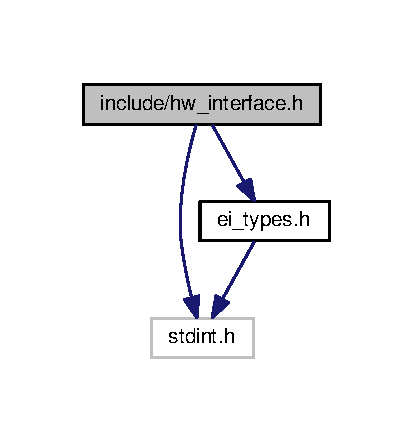
\includegraphics[width=198pt]{hw__interface_8h__incl}
\end{center}
\end{figure}
\subsection*{Typedefs}
\begin{DoxyCompactItemize}
\item 
typedef void $\ast$ \hyperlink{hw__interface_8h_ad9970ae727c438faaf09c58c5defb796}{ei\+\_\+surface\+\_\+t}\hypertarget{hw__interface_8h_ad9970ae727c438faaf09c58c5defb796}{}\label{hw__interface_8h_ad9970ae727c438faaf09c58c5defb796}

\begin{DoxyCompactList}\small\item\em Surface hidden type. A surface represents a 2 dimentional array of pixels where drawing can be done. The displayed screen itself is represented by a surface, it is accessed by \hyperlink{hw__interface_8h_a91dcf1275fecec719a60dd6dfeca40c6}{hw\+\_\+create\+\_\+window}. Other \char`\"{}offscreen\char`\"{} surfaces can be created by \hyperlink{hw__interface_8h_ae366821139ee34bb8b92cb2257c89adb}{hw\+\_\+surface\+\_\+create}. \end{DoxyCompactList}\end{DoxyCompactItemize}
\subsection*{Functions}
\begin{DoxyCompactItemize}
\item 
void \hyperlink{hw__interface_8h_acf938165e604a675fe09218a1b3cfb5f}{hw\+\_\+init} ()\hypertarget{hw__interface_8h_acf938165e604a675fe09218a1b3cfb5f}{}\label{hw__interface_8h_acf938165e604a675fe09218a1b3cfb5f}

\begin{DoxyCompactList}\small\item\em Initialises access to the low-\/level operating system services. \end{DoxyCompactList}\item 
void \hyperlink{hw__interface_8h_a6e856924f3b4c8966a870e56a3b1dcb1}{hw\+\_\+quit} ()\hypertarget{hw__interface_8h_a6e856924f3b4c8966a870e56a3b1dcb1}{}\label{hw__interface_8h_a6e856924f3b4c8966a870e56a3b1dcb1}

\begin{DoxyCompactList}\small\item\em Closes the access to the low-\/level operating system services. \end{DoxyCompactList}\item 
\hyperlink{hw__interface_8h_ad9970ae727c438faaf09c58c5defb796}{ei\+\_\+surface\+\_\+t} \hyperlink{hw__interface_8h_a91dcf1275fecec719a60dd6dfeca40c6}{hw\+\_\+create\+\_\+window} (\hyperlink{structei__size__t}{ei\+\_\+size\+\_\+t} $\ast$size, const \hyperlink{ei__types_8h_a383b9af13bd6a0a893096ead3c4d8e28}{ei\+\_\+bool\+\_\+t} full\+Screen)
\begin{DoxyCompactList}\small\item\em Opens the main graphical window of the application. \end{DoxyCompactList}\item 
\hyperlink{hw__interface_8h_ad9970ae727c438faaf09c58c5defb796}{ei\+\_\+surface\+\_\+t} \hyperlink{hw__interface_8h_ae366821139ee34bb8b92cb2257c89adb}{hw\+\_\+surface\+\_\+create} (const \hyperlink{hw__interface_8h_ad9970ae727c438faaf09c58c5defb796}{ei\+\_\+surface\+\_\+t} root, const \hyperlink{structei__size__t}{ei\+\_\+size\+\_\+t} $\ast$size)
\begin{DoxyCompactList}\small\item\em Allocates an off-\/screen drawing surface. \end{DoxyCompactList}\item 
void \hyperlink{hw__interface_8h_a97d0cca63330b33140dd40288ae1022b}{hw\+\_\+surface\+\_\+free} (\hyperlink{hw__interface_8h_ad9970ae727c438faaf09c58c5defb796}{ei\+\_\+surface\+\_\+t} surface)
\begin{DoxyCompactList}\small\item\em Frees a surface allocated by \hyperlink{hw__interface_8h_ae366821139ee34bb8b92cb2257c89adb}{hw\+\_\+surface\+\_\+create}. This must be called on an unlocked surface (see \hyperlink{hw__interface_8h_abf4681e5ead295ccf5b3df3ec8adab66}{hw\+\_\+surface\+\_\+unlock}). \end{DoxyCompactList}\item 
void \hyperlink{hw__interface_8h_a1b9b22f29bb9de0b39ea904fd66251be}{hw\+\_\+surface\+\_\+lock} (\hyperlink{hw__interface_8h_ad9970ae727c438faaf09c58c5defb796}{ei\+\_\+surface\+\_\+t} surface)
\begin{DoxyCompactList}\small\item\em Gains exclusive access to a surface. Every call to this function must be matched by a call to \hyperlink{hw__interface_8h_abf4681e5ead295ccf5b3df3ec8adab66}{hw\+\_\+surface\+\_\+unlock}. The address of the pixel buffer may change while the surface is unlocked. Thus, hw\+\_\+surface\+\_\+get\+\_\+buffer must called after each call to this function. \end{DoxyCompactList}\item 
void \hyperlink{hw__interface_8h_abf4681e5ead295ccf5b3df3ec8adab66}{hw\+\_\+surface\+\_\+unlock} (\hyperlink{hw__interface_8h_ad9970ae727c438faaf09c58c5defb796}{ei\+\_\+surface\+\_\+t} surface)
\begin{DoxyCompactList}\small\item\em Releases the exclusive access to a surface that was locked by \hyperlink{hw__interface_8h_a1b9b22f29bb9de0b39ea904fd66251be}{hw\+\_\+surface\+\_\+lock}. \end{DoxyCompactList}\item 
\hyperlink{structei__size__t}{ei\+\_\+size\+\_\+t} \hyperlink{hw__interface_8h_a7b92235ad70d5017c843c66affccdcd2}{hw\+\_\+surface\+\_\+get\+\_\+size} (const \hyperlink{hw__interface_8h_ad9970ae727c438faaf09c58c5defb796}{ei\+\_\+surface\+\_\+t} surface)
\begin{DoxyCompactList}\small\item\em Returns the size of a surface. \end{DoxyCompactList}\item 
void \hyperlink{hw__interface_8h_a99bbeb4f78f8402e07c9c15204d1bd8b}{hw\+\_\+surface\+\_\+update\+\_\+rects} (const \hyperlink{structei__linked__rect__t}{ei\+\_\+linked\+\_\+rect\+\_\+t} $\ast$rects)
\begin{DoxyCompactList}\small\item\em Requests that a list of rectangular regions of the root surface be updated on screen. \end{DoxyCompactList}\item 
\hyperlink{structei__rect__t}{ei\+\_\+rect\+\_\+t} \hyperlink{hw__interface_8h_a6ca488fe7d5e254ffa9d9e332ee76996}{hw\+\_\+surface\+\_\+get\+\_\+rect} (const \hyperlink{hw__interface_8h_ad9970ae727c438faaf09c58c5defb796}{ei\+\_\+surface\+\_\+t} surface)
\begin{DoxyCompactList}\small\item\em Returns the rectangle of a surface (origin and size). \end{DoxyCompactList}\item 
\hyperlink{structei__color__t}{ei\+\_\+color\+\_\+t} \hyperlink{hw__interface_8h_a0123a13f33cc8d3cb2b6d7f9047837be}{hw\+\_\+get\+\_\+pixel} (const \hyperlink{hw__interface_8h_ad9970ae727c438faaf09c58c5defb796}{ei\+\_\+surface\+\_\+t} surface, const \hyperlink{structei__point__t}{ei\+\_\+point\+\_\+t} pos)
\begin{DoxyCompactList}\small\item\em Returns the color of the pixel at pos. \end{DoxyCompactList}\item 
void \hyperlink{hw__interface_8h_a994ff5648aa769308d32d37904143f60}{hw\+\_\+put\+\_\+pixel} (const \hyperlink{hw__interface_8h_ad9970ae727c438faaf09c58c5defb796}{ei\+\_\+surface\+\_\+t} surface, const \hyperlink{structei__point__t}{ei\+\_\+point\+\_\+t} pos, const \hyperlink{structei__color__t}{ei\+\_\+color\+\_\+t} color)
\begin{DoxyCompactList}\small\item\em Draw the pixel of the surface at pos. \end{DoxyCompactList}\item 
\hyperlink{hw__interface_8h_ad9970ae727c438faaf09c58c5defb796}{ei\+\_\+surface\+\_\+t} \hyperlink{hw__interface_8h_a80b2e2d3270b08b2b83da0e2132e0595}{hw\+\_\+image\+\_\+load} (const char $\ast$filename)
\begin{DoxyCompactList}\small\item\em Creates a surface and loads into it an image read from a file. The caller is responsible to release this surface (\hyperlink{hw__interface_8h_a97d0cca63330b33140dd40288ae1022b}{hw\+\_\+surface\+\_\+free}) when it is no more needed. \end{DoxyCompactList}\item 
\hyperlink{ei__types_8h_a22c8198e4d641e4bc67bb17f9c6bcda7}{ei\+\_\+font\+\_\+t} \hyperlink{hw__interface_8h_a9c6b86bcbcdd0b3e590e1e33fcf893d7}{hw\+\_\+text\+\_\+font\+\_\+create} (const char $\ast$filename, int size)
\begin{DoxyCompactList}\small\item\em Creates a font that can be used to render text. The font must be freed by calling \hyperlink{hw__interface_8h_a2ac46d37db4c40adc10e3afb137f9f02}{hw\+\_\+text\+\_\+font\+\_\+free}. \end{DoxyCompactList}\item 
void \hyperlink{hw__interface_8h_a2ac46d37db4c40adc10e3afb137f9f02}{hw\+\_\+text\+\_\+font\+\_\+free} (\hyperlink{ei__types_8h_a22c8198e4d641e4bc67bb17f9c6bcda7}{ei\+\_\+font\+\_\+t} font)
\begin{DoxyCompactList}\small\item\em Frees a font created by \hyperlink{hw__interface_8h_a9c6b86bcbcdd0b3e590e1e33fcf893d7}{hw\+\_\+text\+\_\+font\+\_\+create}. \end{DoxyCompactList}\item 
void \hyperlink{hw__interface_8h_a0dd8c0a9599e8cf6f2839bbb049d9358}{hw\+\_\+text\+\_\+compute\+\_\+size} (const char $\ast$text, const \hyperlink{ei__types_8h_a22c8198e4d641e4bc67bb17f9c6bcda7}{ei\+\_\+font\+\_\+t} font, int $\ast$width, int $\ast$height)
\begin{DoxyCompactList}\small\item\em Computes the size of a text surface givent the font and the text. \end{DoxyCompactList}\item 
\hyperlink{hw__interface_8h_ad9970ae727c438faaf09c58c5defb796}{ei\+\_\+surface\+\_\+t} \hyperlink{hw__interface_8h_a806521541c5a5a80fbf43105270919e4}{hw\+\_\+text\+\_\+create\+\_\+surface} (const char $\ast$text, const \hyperlink{ei__types_8h_a22c8198e4d641e4bc67bb17f9c6bcda7}{ei\+\_\+font\+\_\+t} font, const \hyperlink{structei__color__t}{ei\+\_\+color\+\_\+t} $\ast$color)
\begin{DoxyCompactList}\small\item\em Creates a surface containing a text. The size of the created surface is just big enough to contain the text. The caller is responsible to release this surface (\hyperlink{hw__interface_8h_a97d0cca63330b33140dd40288ae1022b}{hw\+\_\+surface\+\_\+free}) when it is no more needed. \end{DoxyCompactList}\item 
void \hyperlink{hw__interface_8h_a4b14c99c55a848a7f9ea69545a151c56}{hw\+\_\+wait} (int s\+\_\+delay)
\begin{DoxyCompactList}\small\item\em Waits for the specified number of seconds. This tells the system to pause the current thread for the given amount of time. \end{DoxyCompactList}\item 
void \hyperlink{hw__interface_8h_a512ddccf5f945ac12df4b5e226b2a974}{hw\+\_\+event\+\_\+wait\+\_\+next} (struct \hyperlink{structei__event__t}{ei\+\_\+event\+\_\+t} $\ast$event)
\begin{DoxyCompactList}\small\item\em Lets this processus sleep until a new event is available. \end{DoxyCompactList}\item 
\hyperlink{ei__types_8h_a383b9af13bd6a0a893096ead3c4d8e28}{ei\+\_\+bool\+\_\+t} \hyperlink{hw__interface_8h_a1a1671a4990e4fa625693e8fe7536a1e}{hw\+\_\+event\+\_\+post\+\_\+app} (void $\ast$user\+\_\+param)
\begin{DoxyCompactList}\small\item\em Put an application-\/generated event on the event queue. This will cause \hyperlink{hw__interface_8h_a512ddccf5f945ac12df4b5e226b2a974}{hw\+\_\+event\+\_\+wait\+\_\+next} to wake. \end{DoxyCompactList}\item 
double \hyperlink{hw__interface_8h_a55b51924e6fa16839af0576bc8886c02}{hw\+\_\+now} ()
\begin{DoxyCompactList}\small\item\em Returns the number of seconds since the library was initialised by \hyperlink{hw__interface_8h_acf938165e604a675fe09218a1b3cfb5f}{hw\+\_\+init}. Can be used to measure elpased time between to calls. \end{DoxyCompactList}\end{DoxyCompactItemize}
\subsection*{Variables}
\begin{DoxyCompactItemize}
\item 
const int {\bfseries E\+I\+\_\+\+M\+O\+U\+S\+E\+B\+U\+T\+T\+O\+N\+\_\+\+L\+E\+FT}\hypertarget{hw__interface_8h_a026cb381ddcadffd54b5da73d782dea2}{}\label{hw__interface_8h_a026cb381ddcadffd54b5da73d782dea2}

\item 
const int {\bfseries E\+I\+\_\+\+M\+O\+U\+S\+E\+B\+U\+T\+T\+O\+N\+\_\+\+M\+I\+D\+D\+LE}\hypertarget{hw__interface_8h_a18a48d087980072d755e0c585454c48b}{}\label{hw__interface_8h_a18a48d087980072d755e0c585454c48b}

\item 
const int {\bfseries E\+I\+\_\+\+M\+O\+U\+S\+E\+B\+U\+T\+T\+O\+N\+\_\+\+R\+I\+G\+HT}\hypertarget{hw__interface_8h_add78e49422c7326a48963b9f288da47c}{}\label{hw__interface_8h_add78e49422c7326a48963b9f288da47c}

\end{DoxyCompactItemize}


\subsection{Detailed Description}
Low level interface with the graphic hadware. This interface is based on the S\+DL library. 

Created by François Bérard on 30.\+12.\+11. Copyright 2011 Ensimag. All rights reserved. 

\subsection{Function Documentation}
\index{hw\+\_\+interface.\+h@{hw\+\_\+interface.\+h}!hw\+\_\+create\+\_\+window@{hw\+\_\+create\+\_\+window}}
\index{hw\+\_\+create\+\_\+window@{hw\+\_\+create\+\_\+window}!hw\+\_\+interface.\+h@{hw\+\_\+interface.\+h}}
\subsubsection[{\texorpdfstring{hw\+\_\+create\+\_\+window(ei\+\_\+size\+\_\+t $\ast$size, const ei\+\_\+bool\+\_\+t full\+Screen)}{hw_create_window(ei_size_t *size, const ei_bool_t fullScreen)}}]{\setlength{\rightskip}{0pt plus 5cm}{\bf ei\+\_\+surface\+\_\+t} hw\+\_\+create\+\_\+window (
\begin{DoxyParamCaption}
\item[{{\bf ei\+\_\+size\+\_\+t} $\ast$}]{size, }
\item[{const {\bf ei\+\_\+bool\+\_\+t}}]{full\+Screen}
\end{DoxyParamCaption}
)}\hypertarget{hw__interface_8h_a91dcf1275fecec719a60dd6dfeca40c6}{}\label{hw__interface_8h_a91dcf1275fecec719a60dd6dfeca40c6}


Opens the main graphical window of the application. 


\begin{DoxyParams}{Parameters}
{\em size} & Number of horizontal and vertical pixels. \\
\hline
{\em full\+Screen} & If true, opens the window in full screen. Otherwise opens a floating window.\\
\hline
\end{DoxyParams}
\begin{DoxyReturn}{Returns}
The unlocked drawing surface (see \hyperlink{hw__interface_8h_a1b9b22f29bb9de0b39ea904fd66251be}{hw\+\_\+surface\+\_\+lock}). This surface should not be freed by calling \hyperlink{hw__interface_8h_a97d0cca63330b33140dd40288ae1022b}{hw\+\_\+surface\+\_\+free}, it is freed when releasing access to the low-\/level services by calling \hyperlink{hw__interface_8h_a6e856924f3b4c8966a870e56a3b1dcb1}{hw\+\_\+quit}. 
\end{DoxyReturn}
\index{hw\+\_\+interface.\+h@{hw\+\_\+interface.\+h}!hw\+\_\+event\+\_\+post\+\_\+app@{hw\+\_\+event\+\_\+post\+\_\+app}}
\index{hw\+\_\+event\+\_\+post\+\_\+app@{hw\+\_\+event\+\_\+post\+\_\+app}!hw\+\_\+interface.\+h@{hw\+\_\+interface.\+h}}
\subsubsection[{\texorpdfstring{hw\+\_\+event\+\_\+post\+\_\+app(void $\ast$user\+\_\+param)}{hw_event_post_app(void *user_param)}}]{\setlength{\rightskip}{0pt plus 5cm}{\bf ei\+\_\+bool\+\_\+t} hw\+\_\+event\+\_\+post\+\_\+app (
\begin{DoxyParamCaption}
\item[{void $\ast$}]{user\+\_\+param}
\end{DoxyParamCaption}
)}\hypertarget{hw__interface_8h_a1a1671a4990e4fa625693e8fe7536a1e}{}\label{hw__interface_8h_a1a1671a4990e4fa625693e8fe7536a1e}


Put an application-\/generated event on the event queue. This will cause \hyperlink{hw__interface_8h_a512ddccf5f945ac12df4b5e226b2a974}{hw\+\_\+event\+\_\+wait\+\_\+next} to wake. 


\begin{DoxyParams}{Parameters}
{\em user\+\_\+param} & The user parameter that will be retrievable in the event. \\
\hline
\end{DoxyParams}
\index{hw\+\_\+interface.\+h@{hw\+\_\+interface.\+h}!hw\+\_\+event\+\_\+wait\+\_\+next@{hw\+\_\+event\+\_\+wait\+\_\+next}}
\index{hw\+\_\+event\+\_\+wait\+\_\+next@{hw\+\_\+event\+\_\+wait\+\_\+next}!hw\+\_\+interface.\+h@{hw\+\_\+interface.\+h}}
\subsubsection[{\texorpdfstring{hw\+\_\+event\+\_\+wait\+\_\+next(struct ei\+\_\+event\+\_\+t $\ast$event)}{hw_event_wait_next(struct ei_event_t *event)}}]{\setlength{\rightskip}{0pt plus 5cm}void hw\+\_\+event\+\_\+wait\+\_\+next (
\begin{DoxyParamCaption}
\item[{struct {\bf ei\+\_\+event\+\_\+t} $\ast$}]{event}
\end{DoxyParamCaption}
)}\hypertarget{hw__interface_8h_a512ddccf5f945ac12df4b5e226b2a974}{}\label{hw__interface_8h_a512ddccf5f945ac12df4b5e226b2a974}


Lets this processus sleep until a new event is available. 


\begin{DoxyParams}{Parameters}
{\em event} & Where to store the new event. The structure must be allocated by the caller. On return, the structure is filled with informations about the new event. \\
\hline
\end{DoxyParams}
\index{hw\+\_\+interface.\+h@{hw\+\_\+interface.\+h}!hw\+\_\+get\+\_\+pixel@{hw\+\_\+get\+\_\+pixel}}
\index{hw\+\_\+get\+\_\+pixel@{hw\+\_\+get\+\_\+pixel}!hw\+\_\+interface.\+h@{hw\+\_\+interface.\+h}}
\subsubsection[{\texorpdfstring{hw\+\_\+get\+\_\+pixel(const ei\+\_\+surface\+\_\+t surface, const ei\+\_\+point\+\_\+t pos)}{hw_get_pixel(const ei_surface_t surface, const ei_point_t pos)}}]{\setlength{\rightskip}{0pt plus 5cm}{\bf ei\+\_\+color\+\_\+t} hw\+\_\+get\+\_\+pixel (
\begin{DoxyParamCaption}
\item[{const {\bf ei\+\_\+surface\+\_\+t}}]{surface, }
\item[{const {\bf ei\+\_\+point\+\_\+t}}]{pos}
\end{DoxyParamCaption}
)}\hypertarget{hw__interface_8h_a0123a13f33cc8d3cb2b6d7f9047837be}{}\label{hw__interface_8h_a0123a13f33cc8d3cb2b6d7f9047837be}


Returns the color of the pixel at pos. 


\begin{DoxyParams}{Parameters}
{\em surface} & The surface on which to draw.\\
\hline
{\em pos} & The position at which to draw.\\
\hline
{\em color} & The color to draw.\\
\hline
\end{DoxyParams}
\begin{DoxyReturn}{Returns}
The color of teh pixel. 
\end{DoxyReturn}
\index{hw\+\_\+interface.\+h@{hw\+\_\+interface.\+h}!hw\+\_\+image\+\_\+load@{hw\+\_\+image\+\_\+load}}
\index{hw\+\_\+image\+\_\+load@{hw\+\_\+image\+\_\+load}!hw\+\_\+interface.\+h@{hw\+\_\+interface.\+h}}
\subsubsection[{\texorpdfstring{hw\+\_\+image\+\_\+load(const char $\ast$filename)}{hw_image_load(const char *filename)}}]{\setlength{\rightskip}{0pt plus 5cm}{\bf ei\+\_\+surface\+\_\+t} hw\+\_\+image\+\_\+load (
\begin{DoxyParamCaption}
\item[{const char $\ast$}]{filename}
\end{DoxyParamCaption}
)}\hypertarget{hw__interface_8h_a80b2e2d3270b08b2b83da0e2132e0595}{}\label{hw__interface_8h_a80b2e2d3270b08b2b83da0e2132e0595}


Creates a surface and loads into it an image read from a file. The caller is responsible to release this surface (\hyperlink{hw__interface_8h_a97d0cca63330b33140dd40288ae1022b}{hw\+\_\+surface\+\_\+free}) when it is no more needed. 


\begin{DoxyParams}{Parameters}
{\em filename} & The name of the file containing the image. The file can be .bmp, .png, .jpg, .tga\\
\hline
\end{DoxyParams}
\begin{DoxyReturn}{Returns}
A new unlocked surface containing the image. 
\end{DoxyReturn}
\index{hw\+\_\+interface.\+h@{hw\+\_\+interface.\+h}!hw\+\_\+now@{hw\+\_\+now}}
\index{hw\+\_\+now@{hw\+\_\+now}!hw\+\_\+interface.\+h@{hw\+\_\+interface.\+h}}
\subsubsection[{\texorpdfstring{hw\+\_\+now()}{hw_now()}}]{\setlength{\rightskip}{0pt plus 5cm}double hw\+\_\+now (
\begin{DoxyParamCaption}
{}
\end{DoxyParamCaption}
)}\hypertarget{hw__interface_8h_a55b51924e6fa16839af0576bc8886c02}{}\label{hw__interface_8h_a55b51924e6fa16839af0576bc8886c02}


Returns the number of seconds since the library was initialised by \hyperlink{hw__interface_8h_acf938165e604a675fe09218a1b3cfb5f}{hw\+\_\+init}. Can be used to measure elpased time between to calls. 

\begin{DoxyReturn}{Returns}
The current time, in seconds. 
\end{DoxyReturn}
\index{hw\+\_\+interface.\+h@{hw\+\_\+interface.\+h}!hw\+\_\+put\+\_\+pixel@{hw\+\_\+put\+\_\+pixel}}
\index{hw\+\_\+put\+\_\+pixel@{hw\+\_\+put\+\_\+pixel}!hw\+\_\+interface.\+h@{hw\+\_\+interface.\+h}}
\subsubsection[{\texorpdfstring{hw\+\_\+put\+\_\+pixel(const ei\+\_\+surface\+\_\+t surface, const ei\+\_\+point\+\_\+t pos, const ei\+\_\+color\+\_\+t color)}{hw_put_pixel(const ei_surface_t surface, const ei_point_t pos, const ei_color_t color)}}]{\setlength{\rightskip}{0pt plus 5cm}void hw\+\_\+put\+\_\+pixel (
\begin{DoxyParamCaption}
\item[{const {\bf ei\+\_\+surface\+\_\+t}}]{surface, }
\item[{const {\bf ei\+\_\+point\+\_\+t}}]{pos, }
\item[{const {\bf ei\+\_\+color\+\_\+t}}]{color}
\end{DoxyParamCaption}
)}\hypertarget{hw__interface_8h_a994ff5648aa769308d32d37904143f60}{}\label{hw__interface_8h_a994ff5648aa769308d32d37904143f60}


Draw the pixel of the surface at pos. 


\begin{DoxyParams}{Parameters}
{\em surface} & The surface on which to draw.\\
\hline
{\em pos} & The position at which to draw.\\
\hline
{\em color} & The color to draw. \\
\hline
\end{DoxyParams}
\index{hw\+\_\+interface.\+h@{hw\+\_\+interface.\+h}!hw\+\_\+surface\+\_\+create@{hw\+\_\+surface\+\_\+create}}
\index{hw\+\_\+surface\+\_\+create@{hw\+\_\+surface\+\_\+create}!hw\+\_\+interface.\+h@{hw\+\_\+interface.\+h}}
\subsubsection[{\texorpdfstring{hw\+\_\+surface\+\_\+create(const ei\+\_\+surface\+\_\+t root, const ei\+\_\+size\+\_\+t $\ast$size)}{hw_surface_create(const ei_surface_t root, const ei_size_t *size)}}]{\setlength{\rightskip}{0pt plus 5cm}{\bf ei\+\_\+surface\+\_\+t} hw\+\_\+surface\+\_\+create (
\begin{DoxyParamCaption}
\item[{const {\bf ei\+\_\+surface\+\_\+t}}]{root, }
\item[{const {\bf ei\+\_\+size\+\_\+t} $\ast$}]{size}
\end{DoxyParamCaption}
)}\hypertarget{hw__interface_8h_ae366821139ee34bb8b92cb2257c89adb}{}\label{hw__interface_8h_ae366821139ee34bb8b92cb2257c89adb}


Allocates an off-\/screen drawing surface. 


\begin{DoxyParams}{Parameters}
{\em root} & The root window which channel indices will be used. This insures that the offscreen uses the same channel indices (Red, Green, Blue, Alpha) as the root surface. \\
\hline
{\em size} & Number of horizontal and vertical pixels. \\
\hline
{\em force\+\_\+alpha} & If true, then the returned surface will use an alpha channel regardless of root having an alpha channel or not.\\
\hline
\end{DoxyParams}
\begin{DoxyReturn}{Returns}
The unlocked drawing surface (see \hyperlink{hw__interface_8h_a1b9b22f29bb9de0b39ea904fd66251be}{hw\+\_\+surface\+\_\+lock}). The surface should be freed by calling \hyperlink{hw__interface_8h_a97d0cca63330b33140dd40288ae1022b}{hw\+\_\+surface\+\_\+free}. 
\end{DoxyReturn}
\index{hw\+\_\+interface.\+h@{hw\+\_\+interface.\+h}!hw\+\_\+surface\+\_\+free@{hw\+\_\+surface\+\_\+free}}
\index{hw\+\_\+surface\+\_\+free@{hw\+\_\+surface\+\_\+free}!hw\+\_\+interface.\+h@{hw\+\_\+interface.\+h}}
\subsubsection[{\texorpdfstring{hw\+\_\+surface\+\_\+free(ei\+\_\+surface\+\_\+t surface)}{hw_surface_free(ei_surface_t surface)}}]{\setlength{\rightskip}{0pt plus 5cm}void hw\+\_\+surface\+\_\+free (
\begin{DoxyParamCaption}
\item[{{\bf ei\+\_\+surface\+\_\+t}}]{surface}
\end{DoxyParamCaption}
)}\hypertarget{hw__interface_8h_a97d0cca63330b33140dd40288ae1022b}{}\label{hw__interface_8h_a97d0cca63330b33140dd40288ae1022b}


Frees a surface allocated by \hyperlink{hw__interface_8h_ae366821139ee34bb8b92cb2257c89adb}{hw\+\_\+surface\+\_\+create}. This must be called on an unlocked surface (see \hyperlink{hw__interface_8h_abf4681e5ead295ccf5b3df3ec8adab66}{hw\+\_\+surface\+\_\+unlock}). 


\begin{DoxyParams}{Parameters}
{\em surface} & The surface to be freed. \\
\hline
\end{DoxyParams}
\index{hw\+\_\+interface.\+h@{hw\+\_\+interface.\+h}!hw\+\_\+surface\+\_\+get\+\_\+rect@{hw\+\_\+surface\+\_\+get\+\_\+rect}}
\index{hw\+\_\+surface\+\_\+get\+\_\+rect@{hw\+\_\+surface\+\_\+get\+\_\+rect}!hw\+\_\+interface.\+h@{hw\+\_\+interface.\+h}}
\subsubsection[{\texorpdfstring{hw\+\_\+surface\+\_\+get\+\_\+rect(const ei\+\_\+surface\+\_\+t surface)}{hw_surface_get_rect(const ei_surface_t surface)}}]{\setlength{\rightskip}{0pt plus 5cm}{\bf ei\+\_\+rect\+\_\+t} hw\+\_\+surface\+\_\+get\+\_\+rect (
\begin{DoxyParamCaption}
\item[{const {\bf ei\+\_\+surface\+\_\+t}}]{surface}
\end{DoxyParamCaption}
)}\hypertarget{hw__interface_8h_a6ca488fe7d5e254ffa9d9e332ee76996}{}\label{hw__interface_8h_a6ca488fe7d5e254ffa9d9e332ee76996}


Returns the rectangle of a surface (origin and size). 


\begin{DoxyParams}{Parameters}
{\em surface} & The surface which rectangle is requested.\\
\hline
\end{DoxyParams}
\begin{DoxyReturn}{Returns}
The rectangle of the surface. 
\end{DoxyReturn}
\index{hw\+\_\+interface.\+h@{hw\+\_\+interface.\+h}!hw\+\_\+surface\+\_\+get\+\_\+size@{hw\+\_\+surface\+\_\+get\+\_\+size}}
\index{hw\+\_\+surface\+\_\+get\+\_\+size@{hw\+\_\+surface\+\_\+get\+\_\+size}!hw\+\_\+interface.\+h@{hw\+\_\+interface.\+h}}
\subsubsection[{\texorpdfstring{hw\+\_\+surface\+\_\+get\+\_\+size(const ei\+\_\+surface\+\_\+t surface)}{hw_surface_get_size(const ei_surface_t surface)}}]{\setlength{\rightskip}{0pt plus 5cm}{\bf ei\+\_\+size\+\_\+t} hw\+\_\+surface\+\_\+get\+\_\+size (
\begin{DoxyParamCaption}
\item[{const {\bf ei\+\_\+surface\+\_\+t}}]{surface}
\end{DoxyParamCaption}
)}\hypertarget{hw__interface_8h_a7b92235ad70d5017c843c66affccdcd2}{}\label{hw__interface_8h_a7b92235ad70d5017c843c66affccdcd2}


Returns the size of a surface. 


\begin{DoxyParams}{Parameters}
{\em surface} & The surface which size is requested.\\
\hline
\end{DoxyParams}
\begin{DoxyReturn}{Returns}
The size of the surface. 
\end{DoxyReturn}
\index{hw\+\_\+interface.\+h@{hw\+\_\+interface.\+h}!hw\+\_\+surface\+\_\+lock@{hw\+\_\+surface\+\_\+lock}}
\index{hw\+\_\+surface\+\_\+lock@{hw\+\_\+surface\+\_\+lock}!hw\+\_\+interface.\+h@{hw\+\_\+interface.\+h}}
\subsubsection[{\texorpdfstring{hw\+\_\+surface\+\_\+lock(ei\+\_\+surface\+\_\+t surface)}{hw_surface_lock(ei_surface_t surface)}}]{\setlength{\rightskip}{0pt plus 5cm}void hw\+\_\+surface\+\_\+lock (
\begin{DoxyParamCaption}
\item[{{\bf ei\+\_\+surface\+\_\+t}}]{surface}
\end{DoxyParamCaption}
)}\hypertarget{hw__interface_8h_a1b9b22f29bb9de0b39ea904fd66251be}{}\label{hw__interface_8h_a1b9b22f29bb9de0b39ea904fd66251be}


Gains exclusive access to a surface. Every call to this function must be matched by a call to \hyperlink{hw__interface_8h_abf4681e5ead295ccf5b3df3ec8adab66}{hw\+\_\+surface\+\_\+unlock}. The address of the pixel buffer may change while the surface is unlocked. Thus, hw\+\_\+surface\+\_\+get\+\_\+buffer must called after each call to this function. 


\begin{DoxyParams}{Parameters}
{\em surface} & The surface to lock. \\
\hline
\end{DoxyParams}
\index{hw\+\_\+interface.\+h@{hw\+\_\+interface.\+h}!hw\+\_\+surface\+\_\+unlock@{hw\+\_\+surface\+\_\+unlock}}
\index{hw\+\_\+surface\+\_\+unlock@{hw\+\_\+surface\+\_\+unlock}!hw\+\_\+interface.\+h@{hw\+\_\+interface.\+h}}
\subsubsection[{\texorpdfstring{hw\+\_\+surface\+\_\+unlock(ei\+\_\+surface\+\_\+t surface)}{hw_surface_unlock(ei_surface_t surface)}}]{\setlength{\rightskip}{0pt plus 5cm}void hw\+\_\+surface\+\_\+unlock (
\begin{DoxyParamCaption}
\item[{{\bf ei\+\_\+surface\+\_\+t}}]{surface}
\end{DoxyParamCaption}
)}\hypertarget{hw__interface_8h_abf4681e5ead295ccf5b3df3ec8adab66}{}\label{hw__interface_8h_abf4681e5ead295ccf5b3df3ec8adab66}


Releases the exclusive access to a surface that was locked by \hyperlink{hw__interface_8h_a1b9b22f29bb9de0b39ea904fd66251be}{hw\+\_\+surface\+\_\+lock}. 


\begin{DoxyParams}{Parameters}
{\em surface} & The surface to unlock. \\
\hline
\end{DoxyParams}
\index{hw\+\_\+interface.\+h@{hw\+\_\+interface.\+h}!hw\+\_\+surface\+\_\+update\+\_\+rects@{hw\+\_\+surface\+\_\+update\+\_\+rects}}
\index{hw\+\_\+surface\+\_\+update\+\_\+rects@{hw\+\_\+surface\+\_\+update\+\_\+rects}!hw\+\_\+interface.\+h@{hw\+\_\+interface.\+h}}
\subsubsection[{\texorpdfstring{hw\+\_\+surface\+\_\+update\+\_\+rects(const ei\+\_\+linked\+\_\+rect\+\_\+t $\ast$rects)}{hw_surface_update_rects(const ei_linked_rect_t *rects)}}]{\setlength{\rightskip}{0pt plus 5cm}void hw\+\_\+surface\+\_\+update\+\_\+rects (
\begin{DoxyParamCaption}
\item[{const {\bf ei\+\_\+linked\+\_\+rect\+\_\+t} $\ast$}]{rects}
\end{DoxyParamCaption}
)}\hypertarget{hw__interface_8h_a99bbeb4f78f8402e07c9c15204d1bd8b}{}\label{hw__interface_8h_a99bbeb4f78f8402e07c9c15204d1bd8b}


Requests that a list of rectangular regions of the root surface be updated on screen. 


\begin{DoxyParams}{Parameters}
{\em rects} & The list of rectangle to be updated on screen. If N\+U\+LL, then the entire surface is updated. \\
\hline
\end{DoxyParams}
\index{hw\+\_\+interface.\+h@{hw\+\_\+interface.\+h}!hw\+\_\+text\+\_\+compute\+\_\+size@{hw\+\_\+text\+\_\+compute\+\_\+size}}
\index{hw\+\_\+text\+\_\+compute\+\_\+size@{hw\+\_\+text\+\_\+compute\+\_\+size}!hw\+\_\+interface.\+h@{hw\+\_\+interface.\+h}}
\subsubsection[{\texorpdfstring{hw\+\_\+text\+\_\+compute\+\_\+size(const char $\ast$text, const ei\+\_\+font\+\_\+t font, int $\ast$width, int $\ast$height)}{hw_text_compute_size(const char *text, const ei_font_t font, int *width, int *height)}}]{\setlength{\rightskip}{0pt plus 5cm}void hw\+\_\+text\+\_\+compute\+\_\+size (
\begin{DoxyParamCaption}
\item[{const char $\ast$}]{text, }
\item[{const {\bf ei\+\_\+font\+\_\+t}}]{font, }
\item[{int $\ast$}]{width, }
\item[{int $\ast$}]{height}
\end{DoxyParamCaption}
)}\hypertarget{hw__interface_8h_a0dd8c0a9599e8cf6f2839bbb049d9358}{}\label{hw__interface_8h_a0dd8c0a9599e8cf6f2839bbb049d9358}


Computes the size of a text surface givent the font and the text. 


\begin{DoxyParams}{Parameters}
{\em text} & The string of the message. \\
\hline
{\em font} & The font used to render the text. \\
\hline
{\em width,height} & Addresses where to store the computed width and height of the text surface. \\
\hline
\end{DoxyParams}
\index{hw\+\_\+interface.\+h@{hw\+\_\+interface.\+h}!hw\+\_\+text\+\_\+create\+\_\+surface@{hw\+\_\+text\+\_\+create\+\_\+surface}}
\index{hw\+\_\+text\+\_\+create\+\_\+surface@{hw\+\_\+text\+\_\+create\+\_\+surface}!hw\+\_\+interface.\+h@{hw\+\_\+interface.\+h}}
\subsubsection[{\texorpdfstring{hw\+\_\+text\+\_\+create\+\_\+surface(const char $\ast$text, const ei\+\_\+font\+\_\+t font, const ei\+\_\+color\+\_\+t $\ast$color)}{hw_text_create_surface(const char *text, const ei_font_t font, const ei_color_t *color)}}]{\setlength{\rightskip}{0pt plus 5cm}{\bf ei\+\_\+surface\+\_\+t} hw\+\_\+text\+\_\+create\+\_\+surface (
\begin{DoxyParamCaption}
\item[{const char $\ast$}]{text, }
\item[{const {\bf ei\+\_\+font\+\_\+t}}]{font, }
\item[{const {\bf ei\+\_\+color\+\_\+t} $\ast$}]{color}
\end{DoxyParamCaption}
)}\hypertarget{hw__interface_8h_a806521541c5a5a80fbf43105270919e4}{}\label{hw__interface_8h_a806521541c5a5a80fbf43105270919e4}


Creates a surface containing a text. The size of the created surface is just big enough to contain the text. The caller is responsible to release this surface (\hyperlink{hw__interface_8h_a97d0cca63330b33140dd40288ae1022b}{hw\+\_\+surface\+\_\+free}) when it is no more needed. 


\begin{DoxyParams}{Parameters}
{\em text} & The string of the message. \\
\hline
{\em font} & The font used to render the text. \\
\hline
{\em color} & The text color. The alpha parameter is not used. However, the text is rendered with alpha blending to smooth the curves of the letters (anti-\/aliasing).\\
\hline
\end{DoxyParams}
\begin{DoxyReturn}{Returns}
A newly created unlocked surface containing an anti-\/aliased rendering of the text. The anti-\/aliasing is implemented with the alpha channel of the surface\+: pixels on the text\textquotesingle{}s boundaries have some transparency. 
\end{DoxyReturn}
\index{hw\+\_\+interface.\+h@{hw\+\_\+interface.\+h}!hw\+\_\+text\+\_\+font\+\_\+create@{hw\+\_\+text\+\_\+font\+\_\+create}}
\index{hw\+\_\+text\+\_\+font\+\_\+create@{hw\+\_\+text\+\_\+font\+\_\+create}!hw\+\_\+interface.\+h@{hw\+\_\+interface.\+h}}
\subsubsection[{\texorpdfstring{hw\+\_\+text\+\_\+font\+\_\+create(const char $\ast$filename, int size)}{hw_text_font_create(const char *filename, int size)}}]{\setlength{\rightskip}{0pt plus 5cm}{\bf ei\+\_\+font\+\_\+t} hw\+\_\+text\+\_\+font\+\_\+create (
\begin{DoxyParamCaption}
\item[{const char $\ast$}]{filename, }
\item[{int}]{size}
\end{DoxyParamCaption}
)}\hypertarget{hw__interface_8h_a9c6b86bcbcdd0b3e590e1e33fcf893d7}{}\label{hw__interface_8h_a9c6b86bcbcdd0b3e590e1e33fcf893d7}


Creates a font that can be used to render text. The font must be freed by calling \hyperlink{hw__interface_8h_a2ac46d37db4c40adc10e3afb137f9f02}{hw\+\_\+text\+\_\+font\+\_\+free}. 


\begin{DoxyParams}{Parameters}
{\em filename} & The path to the file containing the ttf font definition. Can be relative. \\
\hline
{\em style} & The style of the font (normal, bold, ...). \\
\hline
{\em size} & The size of the characters in pixels.\\
\hline
\end{DoxyParams}
\begin{DoxyReturn}{Returns}
The font. 
\end{DoxyReturn}
\index{hw\+\_\+interface.\+h@{hw\+\_\+interface.\+h}!hw\+\_\+text\+\_\+font\+\_\+free@{hw\+\_\+text\+\_\+font\+\_\+free}}
\index{hw\+\_\+text\+\_\+font\+\_\+free@{hw\+\_\+text\+\_\+font\+\_\+free}!hw\+\_\+interface.\+h@{hw\+\_\+interface.\+h}}
\subsubsection[{\texorpdfstring{hw\+\_\+text\+\_\+font\+\_\+free(ei\+\_\+font\+\_\+t font)}{hw_text_font_free(ei_font_t font)}}]{\setlength{\rightskip}{0pt plus 5cm}void hw\+\_\+text\+\_\+font\+\_\+free (
\begin{DoxyParamCaption}
\item[{{\bf ei\+\_\+font\+\_\+t}}]{font}
\end{DoxyParamCaption}
)}\hypertarget{hw__interface_8h_a2ac46d37db4c40adc10e3afb137f9f02}{}\label{hw__interface_8h_a2ac46d37db4c40adc10e3afb137f9f02}


Frees a font created by \hyperlink{hw__interface_8h_a9c6b86bcbcdd0b3e590e1e33fcf893d7}{hw\+\_\+text\+\_\+font\+\_\+create}. 


\begin{DoxyParams}{Parameters}
{\em font} & The font to be freed. \\
\hline
\end{DoxyParams}
\index{hw\+\_\+interface.\+h@{hw\+\_\+interface.\+h}!hw\+\_\+wait@{hw\+\_\+wait}}
\index{hw\+\_\+wait@{hw\+\_\+wait}!hw\+\_\+interface.\+h@{hw\+\_\+interface.\+h}}
\subsubsection[{\texorpdfstring{hw\+\_\+wait(int s\+\_\+delay)}{hw_wait(int s_delay)}}]{\setlength{\rightskip}{0pt plus 5cm}void hw\+\_\+wait (
\begin{DoxyParamCaption}
\item[{int}]{s\+\_\+delay}
\end{DoxyParamCaption}
)}\hypertarget{hw__interface_8h_a4b14c99c55a848a7f9ea69545a151c56}{}\label{hw__interface_8h_a4b14c99c55a848a7f9ea69545a151c56}


Waits for the specified number of seconds. This tells the system to pause the current thread for the given amount of time. 


\begin{DoxyParams}{Parameters}
{\em s\+\_\+delay} & The amount of time, in seconds, to wait. \\
\hline
\end{DoxyParams}

%--- End generated contents ---

% Index
\backmatter
\newpage
\phantomsection
\clearemptydoublepage
\addcontentsline{toc}{chapter}{Index}
\printindex

\end{document}
